\documentclass[12pt]{report}
\usepackage{graphicx} % Required for inserting images
\usepackage{rotating} % Required for sidewaysfigure
\usepackage{adjustbox} % To adjust regression tables
\usepackage{lscape} % To activate landscape mode
\usepackage{subcaption} % To use subfigures
\usepackage{tikz} % To draw figures
\usepackage{xcolor} % To define custom colors
\usepackage{bbm} % To use indicator function
\usepackage{amsmath} % To use math symbols
\usepackage{appendix} % Optional: for more control over appendices formatting

% Define custom light blue color
\definecolor{lightblue}{RGB}{173, 216, 230}
\definecolor{darkblue}{RGB}{0, 0, 139}
%\usepackage{hyperref} % for cross-references

\usepackage[authordate,backend=biber,maxnames=3,minnames=1, dashed=false, maxbibnames =99]{biblatex-chicago} % Use the Chicago author-date style
\addbibresource{references.bib}
% Customize the citation format to put the year in parentheses
\renewbibmacro*{cite:labelyear+extrayear}{%
  \iffieldundef{labelyear}
    {}
    {\printtext[bibhyperref]{%
       \mkbibparens{\printfield{labelyear}%
       \printfield{extrayear}}}}}



 % Add this line to your preamble
% Language setting
% Replace `English' with e.g. `Spanish' to change the document language
\usepackage[english]{babel}

% Set page size and margins
% Replace `letterpaper' with `a4paper' for UK/EU standard size

\usepackage[top=3cm,bottom=3cm,left=3cm,right=3cm,marginparwidth=1.75cm]{geometry}
	
% Load the setspace package
\usepackage{setspace}
\usepackage{amsmath}
\usepackage{listings}
\usepackage{xcolor}
\usepackage{multirow}
\usepackage{amssymb}
\usepackage{pgfplots}
\usepackage{pgfplotstable}
\usepackage{float}

\usepgfplotslibrary{fillbetween}
\usetikzlibrary{arrows.meta, bending}
\pgfplotsset{compat=newest}
\usetikzlibrary{decorations.markings}
\lstdefinestyle{mystyle}{
    commentstyle=\color{gray},
    keywordstyle=\color{blue},
    numberstyle=\tiny\color{gray},
    stringstyle=\color{purple},
    basicstyle=\ttfamily\footnotesize,
    breakatwhitespace=false,         
    breaklines=true,                 
    captionpos=b,                    
    keepspaces=true,                 
    numbers=left,                    
    numbersep=5pt,                  
    showspaces=false,                
    showstringspaces=false,
    showtabs=false,                  
    tabsize=2
}

\lstset{style=mystyle}

% Useful packages
\usepackage{graphicx}
\usepackage[colorlinks=true, allcolors=black]{hyperref}
\pgfplotsset{width=12cm,compat=1.9}
\setstretch{1.5}



\title{Master Thesis}
\author{Federico Vicentini}
\date{May 2024}

\begin{document}

\begin{titlepage}
    \centering

    \Large UNIVERSITÀ CATTOLICA DEL SACRO CUORE\\
    \Large Campus of Milan\\
    \Large Faculty of Economics\\
    \Large Master program in Economics\\
    \vspace{2cm}
    
\includegraphics[width=0.4\textwidth]{Figures/00-logo.png}\\ 
    \vspace{2cm}
    \Huge Europe's Digitalization and the EDIH initiative: What leads firms to participate? \\

    \vspace{2cm}

    \begin{flushleft}
    \large Supervisor \\
    \large Professor Maria Luisa Mancusi
    \end{flushleft}
    
    \vfill
    
    \hfill
    \begin{minipage}{0.3\textwidth}
        \raggedright
        \large Dissertation by\\
        \large Federico Vicentini\\
        \large Id number: 5112604
    \end{minipage}
    
    \vspace{0.8cm}

    \Large{Academic Year 2023/2024}
    
\end{titlepage}

\newpage

\begin{center}
    \vspace*{\fill}
    \textbf{DISCLAIMER:} For brevity, this document contains only the last two chapters of the thesis, specifically related to the methodology and data used in the analysis, and the results obtained, as well as the conclusions that can be drawn from them. Details on the structure of the full thesis are available in the abstract reported in the following page.
    \vspace*{\fill}
\end{center}

\newpage


\renewcommand{\abstractname}{Abstract}

\begin{abstract}
    \centering{This thesis investigates the drivers of firms' participation in the European Digital Innovation Hubs (EDIH) initiative, launched by the European Commission to enhance digital transformation across Europe, particularly for small and medium-sized enterprises (SMEs). Results from the Digital Maturity Assessment (DMA) survey are presented and analysed. Those provide insights into the current state of firms that participated in the program and their level of digital maturity across various dimensions.

    The main analysis focuses on determining the factors that lead firms to participate in the program. To do this, firms that participated in the EDIH initiative are matched with the ORBIS database to retrieve firm-level financial information. Then, a control group of untreated firms taken from ORBIS is constructed. All the firms in the sample are then geocoded to compute the distance of each from the nearest EDIH hub, and to compute the firm density of the area in which they are located.

    A probit regression model is then used to analyze the drivers of participation, including spatial dimensions, sectoral type, technological intensity, and firm-level characteristics. The results indicate that being closer to an EDIH hub and being located in areas with higher firm density significantly increase participation. Firms in the Manufacturing sector, as well as those in technologically intensive sectors, are more likely to participate in the initiative. This is true also for larger firms, and firms in better financial health.}
\end{abstract}


% \tableofcontents

% \newpage
% \chapter{Introduction}

% \par Digitalization has emerged as a cornerstone of innovation and economic growth in the 21st century. However, Europe is lagging behind its global competitors across every metric that measures digitalization. Neither the public nor the private sector shines in this regard. The newly published \citefield{draghi2024}{title} (also known as the \textit{Draghi report \cite{draghi2024}}) stresses the need to close the digitalization gap, in order to boost productivity in the EU and reach levels of GDP growth on par with those seen in the US.
% \par Even before being noted by the Draghi report though, the European Commission has tried to tackle the issue of lagging digitalization in the EU through the Digital Europe Programme (DIGITAL), launched in 2021 as part of the Multiannual Financial Framework (2021-2027).
% \par One of the multiple initiatives launched through DIGITAL was the creation of a network of European Digital Innovation Hubs, defined as one-stop shops supporting companies (specifically SMEs) and public sector organisations (from now on, PSOs) to respond to digital challenges and become more competitive. Since the start of the EDIH initiative in early 2023, any private company or PSO across Europe can interact with these hubs to receive support for digitalization initiatives.
% \par Aiming to measure the impact of the EDIH initiative itself, the European Commission's Directorate-General for Communications Networks, Content and Technology (also known as DG CNECT) tasked the Joint Research Centre's Digital Economy unit with the design of a Digital Maturity Assessment Tool (DMA). The DMA has been built to give an indication of the effectiveness of the EDIH's intervention on the firms they help. It also provides the firm with information about their relative level of digital maturity compared to their peers across regional and sectoral dimensions.
% \par Every SME or PSO that is a customer of the EDIH network has to complete the DMA survey prior to the EDIH's intervention. The survey is then repeated 1 year later, and 2 years after that. Since the EDIH Network has started operating in early 2023, at the moment most of the firms are still in the infancy stages of intervention.
% \par Unfortunately, at the current stage, it is impossible to have sufficient data to investigate the impact of the EDIH initiative on the firms that participated. Therefore, I will first present the current state of the firms that entered the program, providing information on their current level of digital maturity across the dimensions measured by the DMA. After that, I will investigate the drivers that led this firms to participate in the program itself. 
% \par In order to do this, I am going to match the firms that participated in the program with the ORBIS database, to retrieve firm-level financial information. I will then construct a synthetic control group of untreated firms, taken randomly from the ORBIS database, to compare with the treated sample.
% \par Doing this will give an indication of how much the program is helping its stated target firms, and also make us understand how the program can be made more effective.

% \par This thesis is structured in (N) parts. In the first part, I will present a brief review of the literature on digitalization. The review will mainly focus on studies covering digitalization initiatives by governments, the relevance of firms' characteristics on their level of innovation (for example the role of financial constraints), and the role of Open Innovation ecosystems, such as the EDIH Network.
% \par In the second part, I will take an in-depth look at the EDIH initiative: covering the objective of the program, its birth and development, and its current state 1 year after its official launch.
% \par With the third part, I will explore the Digital Maturity Assessment Tool, presenting the design and structure of the survey. Here I will also present a breakdown of the survey responses, which will give a snapshot of the level of digital maturity and the adoption of specific technologies in the sample of treated firms.
% \par Throughout the fourth part, I will present the bulk of the analysis. Here the main research question, regarding the drivers of participation in the EDIH initiative by firms in the EU, will be explored. The part will be first dealing with how treated firms are matched with ORBIS financial data, then how the sample of control firms is built. After that, a comparison of the two sample is presented, followed by the explanation of the regression model utilized for the analysis and the results from the probit regression.
% \par The fifth and last part will deal with the Discussion of results and conclusions stemming from them, as well as possible avenues of further research.






% \newpage
% \chapter{Literature Review}

% Presenting in this chapter a literature review on the exact subject of this thesis would have been impossible, since the EDIH initiative is too young. Thus, no academic papers cover this specific digitalization initiative by the European Commission.\footnote{The few studies that do exist on the matter are publications from the European Commission's Joint Research Centre, or DG CNECT itself. I am not going to present them here, as they will be treated in the chapter describing the EDIH initiative}
% \par Moreover, few studies deal with the research question the thesis poses, which is concerned with the drivers of firms' participation in public initiatives designed to increase digitalization in the private sector.
% \par Thus, in this chapter I will first present a review of the literature on the topic of innovation more broadly, presenting the main drivers of innovation in firms and also some of the barriers to the production and adoption of innovation. After that, I will move on to present the concept of Open Innovation Ecosystem, such as the EDIH Initiative, which we will cover more in-depth in Chapter 3.

% \newpage

% \section{Innovation, its drivers and barriers}

% \par The study presented in this thesis will be focused mainly on the process of digitalization. However, we can think of digitalization first and foremost as a particular type of innovation, and this is why we will focus our attention on the process of innovation more broadly. 
% \par The economic literature on innovation goes back to Schumpeter's seminal work, \textit{\citetitle{Schumpeter1934} (\citeyear{Schumpeter1934})}. In the book, innovation is defined as the introduction of a new product or production process (or a significant improvement of an existing one). Innovation is conceived as the driver of economic development, through the so-called process of "creative destruction". 
% \par In the 90 years that have passed since the publication of Schumpeter's book, the innovation landscape has changed. As a result of scientific progress, and the process of innovation itself, it has become more costly and more difficult to achieve breakthroughs. \cite{bloom2020} argue that this is true in a vast number of fields of knowledge, noting that in recent years, increasing resources devoted to R\&D did not translate to proportionally higher innovation output.
% \par In this landscape, SMEs face much bigger challenges compared to larger firms. Since R\&D is more costly and less productive than it used to, small firms are incentivized to not invest (or to invest less) on R\&D. In fact, \cite{Crepon1998} showed that the probability of engaging in research for a firm increases with size, market share and diversification for example. Thus, SMEs find themselves at a disadvantageous position: moreover, there is also evidence that financial constraints play a role in determining firms' R\&D decisions, as shown in \cite{Mancusi2014}. In this study, the authors utilize both survey and accounting data from AIDA on firms in Italy. They find that need for external finance has a significant negative effect on the probability of investing in R\&D, pointing to the role of credit constraints in limiting innovation in SMEs. One policy implication of these findings is that easing credit constraints to SMEs is of course, crucial to boosting their R\&D investment.
% \par This can be also one reason to argue for public subsidies to R\&D in firms, especially in countries where Venture Capital is not particularly developed (e.g. European countries). \cite{Czarnitzki2004} look at R\&D subsidies in Germany and find that they significantly influence R\&D expenditure (and also encourage patenting by firms). The study also rejects the possibility of crowding-out effects, which have been instead suggested by other works in the literature.\footnote{A complementary relationship between privately and publicly financed R\&D is indicated by most of the preceding literature; see for reference \cite{david2000}. Successive literature has shown that crowding-out effects can occur in specific contexts, highlighting the importance of firm characteristics as well as the economic environment}


% \par \cite{mina2021} analyzes the SME Instrument, a public initiative by the European Commission designed to help innovative SMEs. They find that although firms that are successful in obtaining the funds are growing faster than the average SME, they nonetheless present lower profit levels, indicating that they were in fact in need of external funding.

% \par However, even when investments in R\&D are there (in the public or the private sector) and yield successful results, there is still the problem of innovation adoption. This is particularly crucial for those technologies which take advantage of positive network effects (and thus necessitate of widespread adoption to achieve their full innovative potential), but is in general true for any innovative technology. In fact, on a macro level, the productivity-enhancing effect of new production technologies can be sizable only if those new methods become widespread.
% \par One recent model of the production of innovation that takes into the account the importance of network effects while also addressing new challenges posed by the new innovation landscape is the Open Innovation model.




% \section{Open Innovation Ecosystems}

% \par The seminal work on the Open Innovation concept comes from a book written by Henry William Chesborough in 2003 (\cite{Chesbrough_2003}). In this book, Open Innovation is defined in contrast to the existing paradigm of Closed Innovation.
% \par Chesborough describes Closed Innovation as a process where:
% \begin{enumerate}
%     \item Companies finance their own private R\&D labs
%     \item These labs produce research leading to new intellectual property
%     \item The intellectual property is developed and capitalized by the company
%     \item Profits from the intellectual property are used to finance further research
% \end{enumerate}
% \par It is clear how this paradigm represents the "classic" way innovation is funded and achieved in a capitalist economic system, as described also in the studies covered in the previous sections. The book however, argues that there are two major factors challenging this paradigm: the growing mobility of skilled professionals, and the growing presence of Venture Capital. These two factors contribute to the escape of intellectual property from the company's control, making the model of Closed Innovation less viable. 
% \par As a new paradigm designed to profit from these new characteristics of the innovation environment, the author proposes to adopt the model of Open Innovation, described as follows:
% \begin{enumerate}
%     \item Firms should utilize both internal and external knowledge in their innovation processes
%     \item To achieve this, a more collaborative knowledge ecosystem is needed: firms and research institutions need to collaborate
%     \item Internal knowledge should be shared in the network, in order to provide for a faster rate of innovation that will in turn benefit also the firm itself
% \end{enumerate}
% \par After publication of the book, subsequent research expanded open innovation, initially focused on large technology-intensive firms, to include the services sector, SMEs and Public Sector Organizations (PSOs). Open Innovation has gradually become central to many regional, national and supranational innovation strategies.
% \par One paper that looks at the effectiveness of the Open Innovation model is \cite{carmonalavado2022}; the study employs fuzzy-set Qualitative Comparative Analysis (fsQCA) to investigate which configurations lead to high performance in innovation among biotech firms in Spain. The authors analyzed data collected through structured questionnaires filled by key figures in the companies, such as CEOs or R\&D managers. The analysis finds that high-performing configurations are characterized by a high number of alliances, diversity of partners, investment in external R\&D, coordination and learning capabilities and complementary organizational assets (e.g. human capital). 
% \par These experimental findings show one of the reasons why public intervention has been thought of as beneficial to Open Innovation: if you need to reach a high number of partners and achieve diversity in those partners, having public-private partnerships is critical.
% \par In fact, public policy has aimed to encourage public-private partnerships, university-industry collaborations and the creation of innovation hubs. The EDIH network is one of these initiatives, that we can define as Open Innovation Ecosystems.\footnote{The specific characteristics of EDIHs as Open Innovation Ecosystem will be covered more in-depth in the chapter on the EDIH Initiative}
% \par Some other notable examples of Open Innovation ecosystems are:
% \begin{itemize}
%     \item Manufacturing USA Institutes and the National Science Foundation's Innovation Corps in the United States of America
%     \item Creative Economy Innovation Centers (CEICs) in South Korea
%     \item Open Innovation Platform in Singapore
%     \item Innovation Superclusters in Canada
%     \item Digital Catapult in the United Kingdom
%     \item Fraunhofer Institutes in Germany
% \end{itemize}
% \par The literature on Open Innovation Ecosystem initiatives is still young, since these are recent programmes, mostly launched in the 2010s and 2020s. However, we can already find a thorough review of the literature on Open Innovation initiatives in \cite{IdrissiFakhreddine2023}. They analyze 99 articles about Open Innovation in SMEs. They find a significant gap in the literature, specifically regarding public policy initiatives to foster OI in SMEs, which is addressed only by 3\% of studies in their sample. 
% \par This thesis will hopefully fill part of that gap, by providing insights into the effectiveness of one specific example of Open Innovation Ecosystem: the EDIH initiative, which I am now going to describe in the next chapter.



% \newpage
% \chapter{The EDIH Initiative}


% \par The European Digital Innovation Hubs (EDIH) initiative, launched by the European Commission in 2021, represents a pivotal step towards enhancing digital transformation across Europe, particularly for small and medium-sized enterprises (SMEs). Established in response to the pressing need for increased digitalization within the EU, where only 20\% of SMEs are considered highly digitized, EDIHs serve as one-stop shops designed to support businesses in the adoption of advanced digital technologies. This chapter will explore the origins of the EDIH network, delineate its main objectives and present descriptive statistics that illustrate the current landscape of EDIHs across Europe. 


% \section{The birth of the EDIH Network}

% \par The EDIH initiative emerged from a broader effort by the European Commission to accelerate digital transformation across the European Union, especially helping SMEs, which have been falling behind on digitalization metrics.
% \par The roots of the program can be found in the \citetitle{dei2016} document (\cite{dei2016}), starting implementation in April 2016, which for the first time created Digital Innovation Hubs (DIHs) across Europe.
% \par DIHs were designed as regional cooperations with multiple participating entities, such as research and technology centres, universities, industry associations, chambers of commerce, incubators/accelerators, regional development
% agencies and vocational training institutes.
% \par These DIHs were precursors to the EDIHs later instituted. These hubs were designed as regional support centers assisting SMEs in digital transformation initiatives by providing access to expertise, test-before-invest opportunities, training, and networking. Their focus was local; as a consequence of this, they were typically financed through national or regional public funds. This of course led to having different levels of support from governments to DIHs across Europe.
% \par It's already clear by this brief description that DIHs were not sufficient to face the challenges of digitalization in the European private sector. Although effective at providing regional support, DIHs struggled to extend their services across regional boundaries, let alone the confines of individual member states. These shortcomings were the main reasons leading to the birth of the EDIH network, to better and improve the effectiveness of Europe's digitalization's initiative. 

% \begin{figure}
%     \centering
%     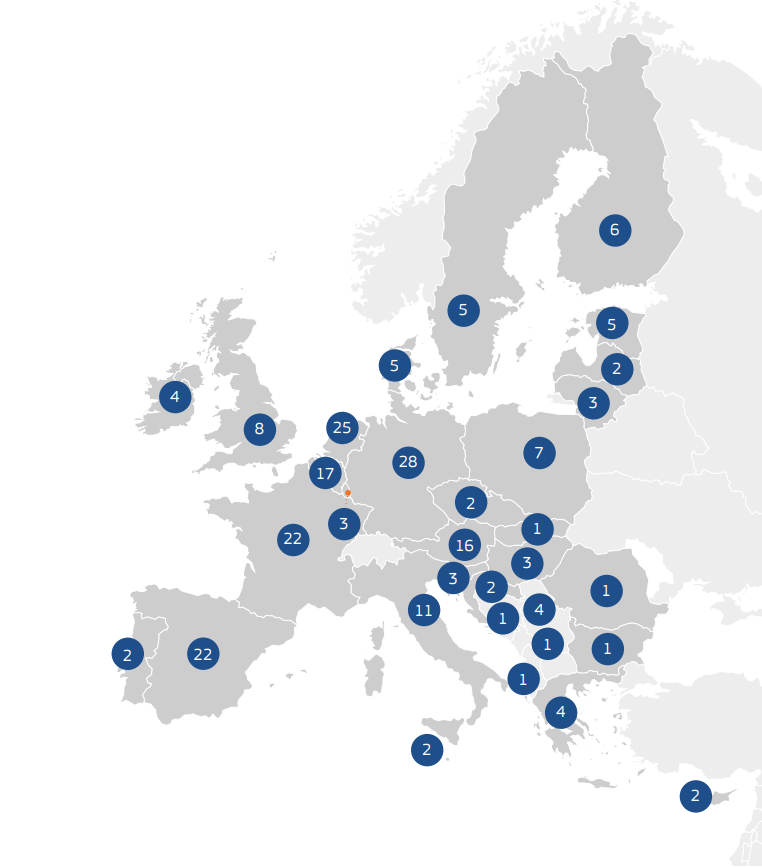
\includegraphics[width=0.5\linewidth]{Figures/01-DIHs_2018.png}
%     \caption{Geographical Distribution by country of Digital Innovation Hubs in Europe as of January 2018, 2 years after the launch of the initiative. Source: \citetitle{dei2018} (\cite{dei2018})}
%     \label{fig:enter-label}
% \end{figure}

% \section{Objectives and functioning of the EDIHs}



% \section{Descriptive statistics on the EDIHs}




% \newpage
% \chapter{The DMA Survey}
% \section{Design and structure of the survey}

% \newpage
% \section{Analysis of the survey responses}


\newpage
% \setcounter{chapter}{4}  % Set the chapter counter to 4
% \setcounter{chapter}{4}  % Set the chapter counter to 4


\newpage
\chapter{What are the drivers of participation?}
\par As we have already discussed, the current state of the EDIH initiative doesn't allow for the analysis of the impact of the policy on firms' digital maturity. The reason leads back to the fact that the program itself is too recent (EDIH activities began in spring of 2023), thus we have no way of knowing what its impact has been, based on firm's financials or even based just on scores from future submissions of the DMA survey\footnote{As of now, we have only a limited number of observations related to T1 issuings of the DMA survey, taken 1 year after the intervention of the EDIH. This initial data indicates a betterment of the Digital Maturity Score, at least in treated firms, even for those sections related to the adoption of specific advanced technologies. However, since the DMA was never submitted to a control group of firms not participating in the program, an analysis of this type would not be able to establish causality.}.

\par However, what we can do is investigate what are the driving factors that are leading firms to participate in the program itself. This can lead us to better understand if the targeting of the policy is working properly, or for example if there are some steps that can be taken in order to increase participation in the program itself. Furthermore, understanding the drivers of participation can also give us insights into the size and sign of the potential bias that can be present in the future analysis of the impact of the program on firms' digital maturity\footnote{For instance, if the analysis were to suggest that one of the positive drivers of participation is firm size, we can hypothesize that when measuring the impact of the policy only on the treated firms, the bias on the effect of digital maturity will be positive, since we can reasonably assume that larger firms can benefit more easily from digitalization initiatives. Conversely, if smaller firms are more likely to participate, the bias might be negative.}.

\par To perform the analysis, I have matched the firms that participated in the EDIH initiative with the ORBIS database to retrieve firm-level financial information (such as their size, country, sector in which they operate, and indicators of financial performance).

\par Once having had the data on treated firms, I have constructed a synthetic control group of untreated firms. These control firms will be selected randomly from the ORBIS database. After constructing the control group, first of all I've compared the treated and control firms to identify any significant differences in their characteristics. This comparison is instrumental to understand the factors that may influence a firm's decision to participate in the EDIH initiative.

\par As an additional information to add on top of country information on where the firms are located, I decided to assess the effect of the distance of firms from the closest EDIH hub. The working hypothesis is that firms that are sited closer to an EDIH hub are more likely to have heard about the program and thus to participate in it. Knowing how distance affects firms' participation can be instrumental in understanding if an expansion in the number of hubs or in their geographical coverage can lead to an increase in participation. Also, to account for the possibility of the effect being confused by areas with a large concentration of firms (which are more likely to have an EDIH hub nearby, and thus more likely to participate), I have computed a measure of firm density. To compute both density and distance, I geocoded the firms' addresses, taken from the ORBIS database or from the DMA survey itself.

\par Finally, I have run a probit regression model to analyze the drivers of participation in the EDIH initiative. The regression model includes various firm-level characteristics as independent variables, and the dependent variable is a dummy variable indicating whether the firm participated in the EDIH initiative.

\par In the following sections, I am going to describe the matching process, the construction of the control group, the treated-control comparison, the geocoding process, and the results of the regression analysis in detail, as well as some robustness checks on those results.

\newpage
\section{Matching of treated firms with ORBIS}

\par To safely match the treated firms with the ORBIS database, I have used the data from the DMA survey replies. Every firm, when submitting the DMA to the Digital Transformation Accelerator platform, has to provide basic company information. Among other things, the database includes firms' legal names, as well as VAT numbers. 

\par These information can be used to match companies with data in ORBIS. However, the DMA tool does not automatically check for invalid VAT numbers, thus some of the reported VAT codes are incorrect. Furthermore, I was relying on WRDS as the website to download the ORBIS database, and WRDS allows for downloading big chunks of data, such as all firms in Europe (or filtering by country, in each European Member State), but only for some specific variables. Among the variables that can be downloaded, there is no VAT code. Thus, I had to rely on company names to match the firms. This is not ideal, since it is possible to have misspellings or different ways of writing the same company name.

\par Thus, to match the treated firms i proceeded in the following way:

\begin{enumerate}
    \item I downloaded the whole universe of firms in ORBIS country by country (for 18 EU Member States where the number of firms participating in the EDIH initiative was the highest), saving them as \texttt{Orbis-COUNTRYCODE-Universe.csv} files.
    \item To have a more efficient code, I loaded the files into memory one country at a time and then, for every country in my DMA database, I computed the Jaro-Winkler distance\footnote{The Jaro-Winkler distance is defined as being equal to 1 minus the Jaro-Winkler similarity: $$dist(JW) = 1 - sim(JW)$$} between that firm's name and that of every company in that country's ORBIS universe, substituting the match every time a smaller distance was found until a threshold of 0.01 was reached\footnote{The threshold of 0.01 was chosen after some trial and error, to minimize the number of false positives while still speeding up the matching process.}. After having done this for every country's ORBIS universe, I saved the results in a .csv file, containing the matched DMA company name, the ORBIS company name, and the corresponding BvD ID number as well as the VAT code from the DMA database.
    \item This allowed me to then download the financial data for the matched firms by searching them in ORBIS through the BvD ID number. I then checked if the VAT code corresponded to the one in the DMA database, by again computing the Jaro-Winkler distance between the 2 strings.\footnote{This was done to make sure that simple misspellings in the input of the VAT code would not cause the matching to be negative.} If the distance was above the threshold, I inspected other variables to check if the match was correct and the VAT code was indeed incorrectly specified.
\end{enumerate}

\par As I was mentioning in the previous chapter on the DMA survey, at the time the analysis was performed the firms in the database were 3204, out of which I was able to match through this procedure 2886 of them. Thus, the percentage of matched firms through this procedure was roughly 90\%. The remaining 10\% of firms were not matched for a number of potential reasons, that can have different implications on the analysis I am going to perform. Potential reasons include:
\begin{itemize}
    \item The firm was not present in the ORBIS database, either due to the firm being too small, too young, or perhaps being located in a country were ORBIS coverage is not perfect.
    \item The firm was present in the ORBIS database, but the name was misspelled or written in a different way, and the Jaro-Winkler distance was too high to match the firm, and instead it matched to a completely different one. This can be the case in particular for firms with shorter names, or sometimes cited with their acronyms.
\end{itemize}
\par I will discuss this more once I present the design of the control group, but for now it is important to note that if the second case is the one driving the majority of the non-matches, since having shorter names or acronyms is not likely to be significantly correlated with any other firm-level characteristics, the bias introduced by the non-matches is likely to be small and negligible.
\par However, if the non-matched firms are mostly belonging to the first case, then we have to keep in mind that it is possible that the matched firms are systematically larger in size, possibly older, and located in country with better ORBIS coverage with respect to the overall sample of firms that participated to the EDIH initiative.


\section{Creating the Control Group}

\par When designing the control group, one has to consider the aim of the analysis it is going to be performed with it. 
\par For example, if the aim is to estimate the impact of the EDIH initiative on firms' digital maturity, the control group should be constructed in a way that it is as similar as possible to the treated group, except for the fact that it did not participate in the program. This is because the aim of the analysis is to estimate the counterfactual: what would have happened to the treated firms if they had not participated in the program. 
\par The case of my analysis however, is a bit different. Since we are trying to estimate the drivers of participation in the program, the control group should be as "agnostic" as possible, the reason being that the best control group for our analysis would be the one that is most representative of the population of firms that could have participated in the program (so, in theory, the whole population of firms in the EU). 
\par Since I cannot have access to the whole population of firms, but only to a subset of them who are reported in the ORBIS database, the best control group is the one that is most representative of the population of firms that are in the ORBIS database. This choice of course has implications, since ORBIS coverage is not the same across all countries, and it is not independent of firm-level characteristics.
\par However, since the treated firms included in the analysis are also only the ones that are present in ORBIS, the bias introduced is likely to be attenuated, since they will share the same selection bias.
\par It should also be noted that if the characteristics leading to better coverage in ORBIS are also the ones leading to participation in the EDIH initiative, the bias introduced by the control group can be positive. 

\par All this taken into account, I have constructed the control group in the following way: I have taken all the firms in the ORBIS database for the 18 selected countries, and picked random BvD IDs with the only constraint that the proportion of firms from a specific country in the synthetic control group should be the same as the proportion of firms from that country in the overall ORBIS database. This was done to ensure that the control group is representative of the population of firms in the ORBIS database.\footnote{Representativeness with respect to other firm-level characteristics was not considered as a constraint. However, the large number of the sampled firms making up the control group should allow for representativeness due to the law of large numbers.}
\par After running this procedure, I had a list of 100000 firms, for which I then downloaded firm-level characteristics from the ORBIS database.
\par After doing this, everything was ready to proceed with the initial comparison between treated and controls.

\section{Treated - Control Comparison}

\par In the table below, I present the results of an initial comparison between treated and control firms. The table shows the mean and median values of the main firm-level characteristics for the two groups, as well as the results of a t-test for the equality of means between the two groups. The t-test is performed for each variable, and the p-value is reported in the last column.

% latex table generated in R 4.4.2 by xtable 1.8-4 package
% Wed Apr  9 18:31:31 2025
\begin{table}[ht]
\centering
\begin{tabular}{lrrr}
  \hline
Statistic & Treated\_0 & Treated\_1 & p\_value \\ 
  \hline
N & 3643.00 & 1249.00 &  \\ 
  Mean\_Employees & 0.03 & 0.09 & 0.00 \\ 
  SD\_Employees & 0.17 & 0.37 &  \\ 
  Mean\_TotalAssets & 14.09 & 15.18 & 0.80 \\ 
  SD\_TotalAssets & 185.97 & 108.15 &  \\ 
  Mean\_LiquidityRatio & 4.15 & 2.33 & 0.00 \\ 
  SD\_LiquidityRatio & 8.41 & 2.90 &  \\ 
  Mean\_Solvency & 37.65 & 50.51 & 0.00 \\ 
  SD\_Solvency & 35.45 & 25.62 &  \\ 
  Mean\_turnover & 9.15 & 16.02 & 0.00 \\ 
  SD\_turnover & 70.39 & 74.00 &  \\ 
   \hline
\end{tabular}
\caption{Comparison between Control Firms (Treated = 0) and Treated ones (Treated = 1), with p-values for the t-test of equal means} 
\end{table}



\par What is immediately noticeable from the first line, where the number of observations for each group is reported, is that both groups shrank in number. This is because not all firms in the ORBIS database have complete financial information, and thus some of them were dropped from the analysis. 
\par To limit this issue, I restricted the analysis to variables that had at most 25\% of \texttt{NAs} observations in each of the two datasets. However, since the observations were retained for the analysis only if all variables had \texttt{non-NA} values, the drop in observations was still significant. The number of treated firms dropped from 2886 to 1249, while the number of control firms dropped from 100000 to 3643 firms\footnote{It should be noted here that the very high sample size for the control group was chosen specifically to make sure that after the drop in observations, the size of the database was still considerably large}.

\par Moving on to the initial comparison of means in the 2 groups, we can see how for the variables showed in the table the means are significantly different. This is confirmed by the t-test, which reports a p-value of 0 for all variables except for total assets, where the p-value is 0.80, probably to the relatively high standard deviation making it difficult to detect a significant difference in means.
\par The comparison highlights something that could be already expected: the firms participating in the EDIH initiative differ significantly from the overall population of firms in ORBIS. However, the sign is what is most interesting: treated firms seem to be having more employees, a better value of the liquidity ratio, higher solvency ratios and turnover (while for total assets the difference from the simple t-test is not significant).

\par We can investigate a little bit further by comparing the distributions of the variables in the treated and control group, variable by variable. this is done in the following figures. There you can see how the treated firms' frequency distribution (in blue) compares to the control group (in red), as well as a kernel density function estimating the distribution of the variable based on the data. In every graph, above you can also see reported the p-value of the KS-test, which tests the null hypothesis that the two distributions are the same. Since the KS-test is a non-parametric test, it allows us to confirm that also in the case of total assets, the two distributions are significantly different.


\begin{figure}[ht]
    \centering
    \begin{subfigure}[b]{0.45\textwidth}
        \centering
        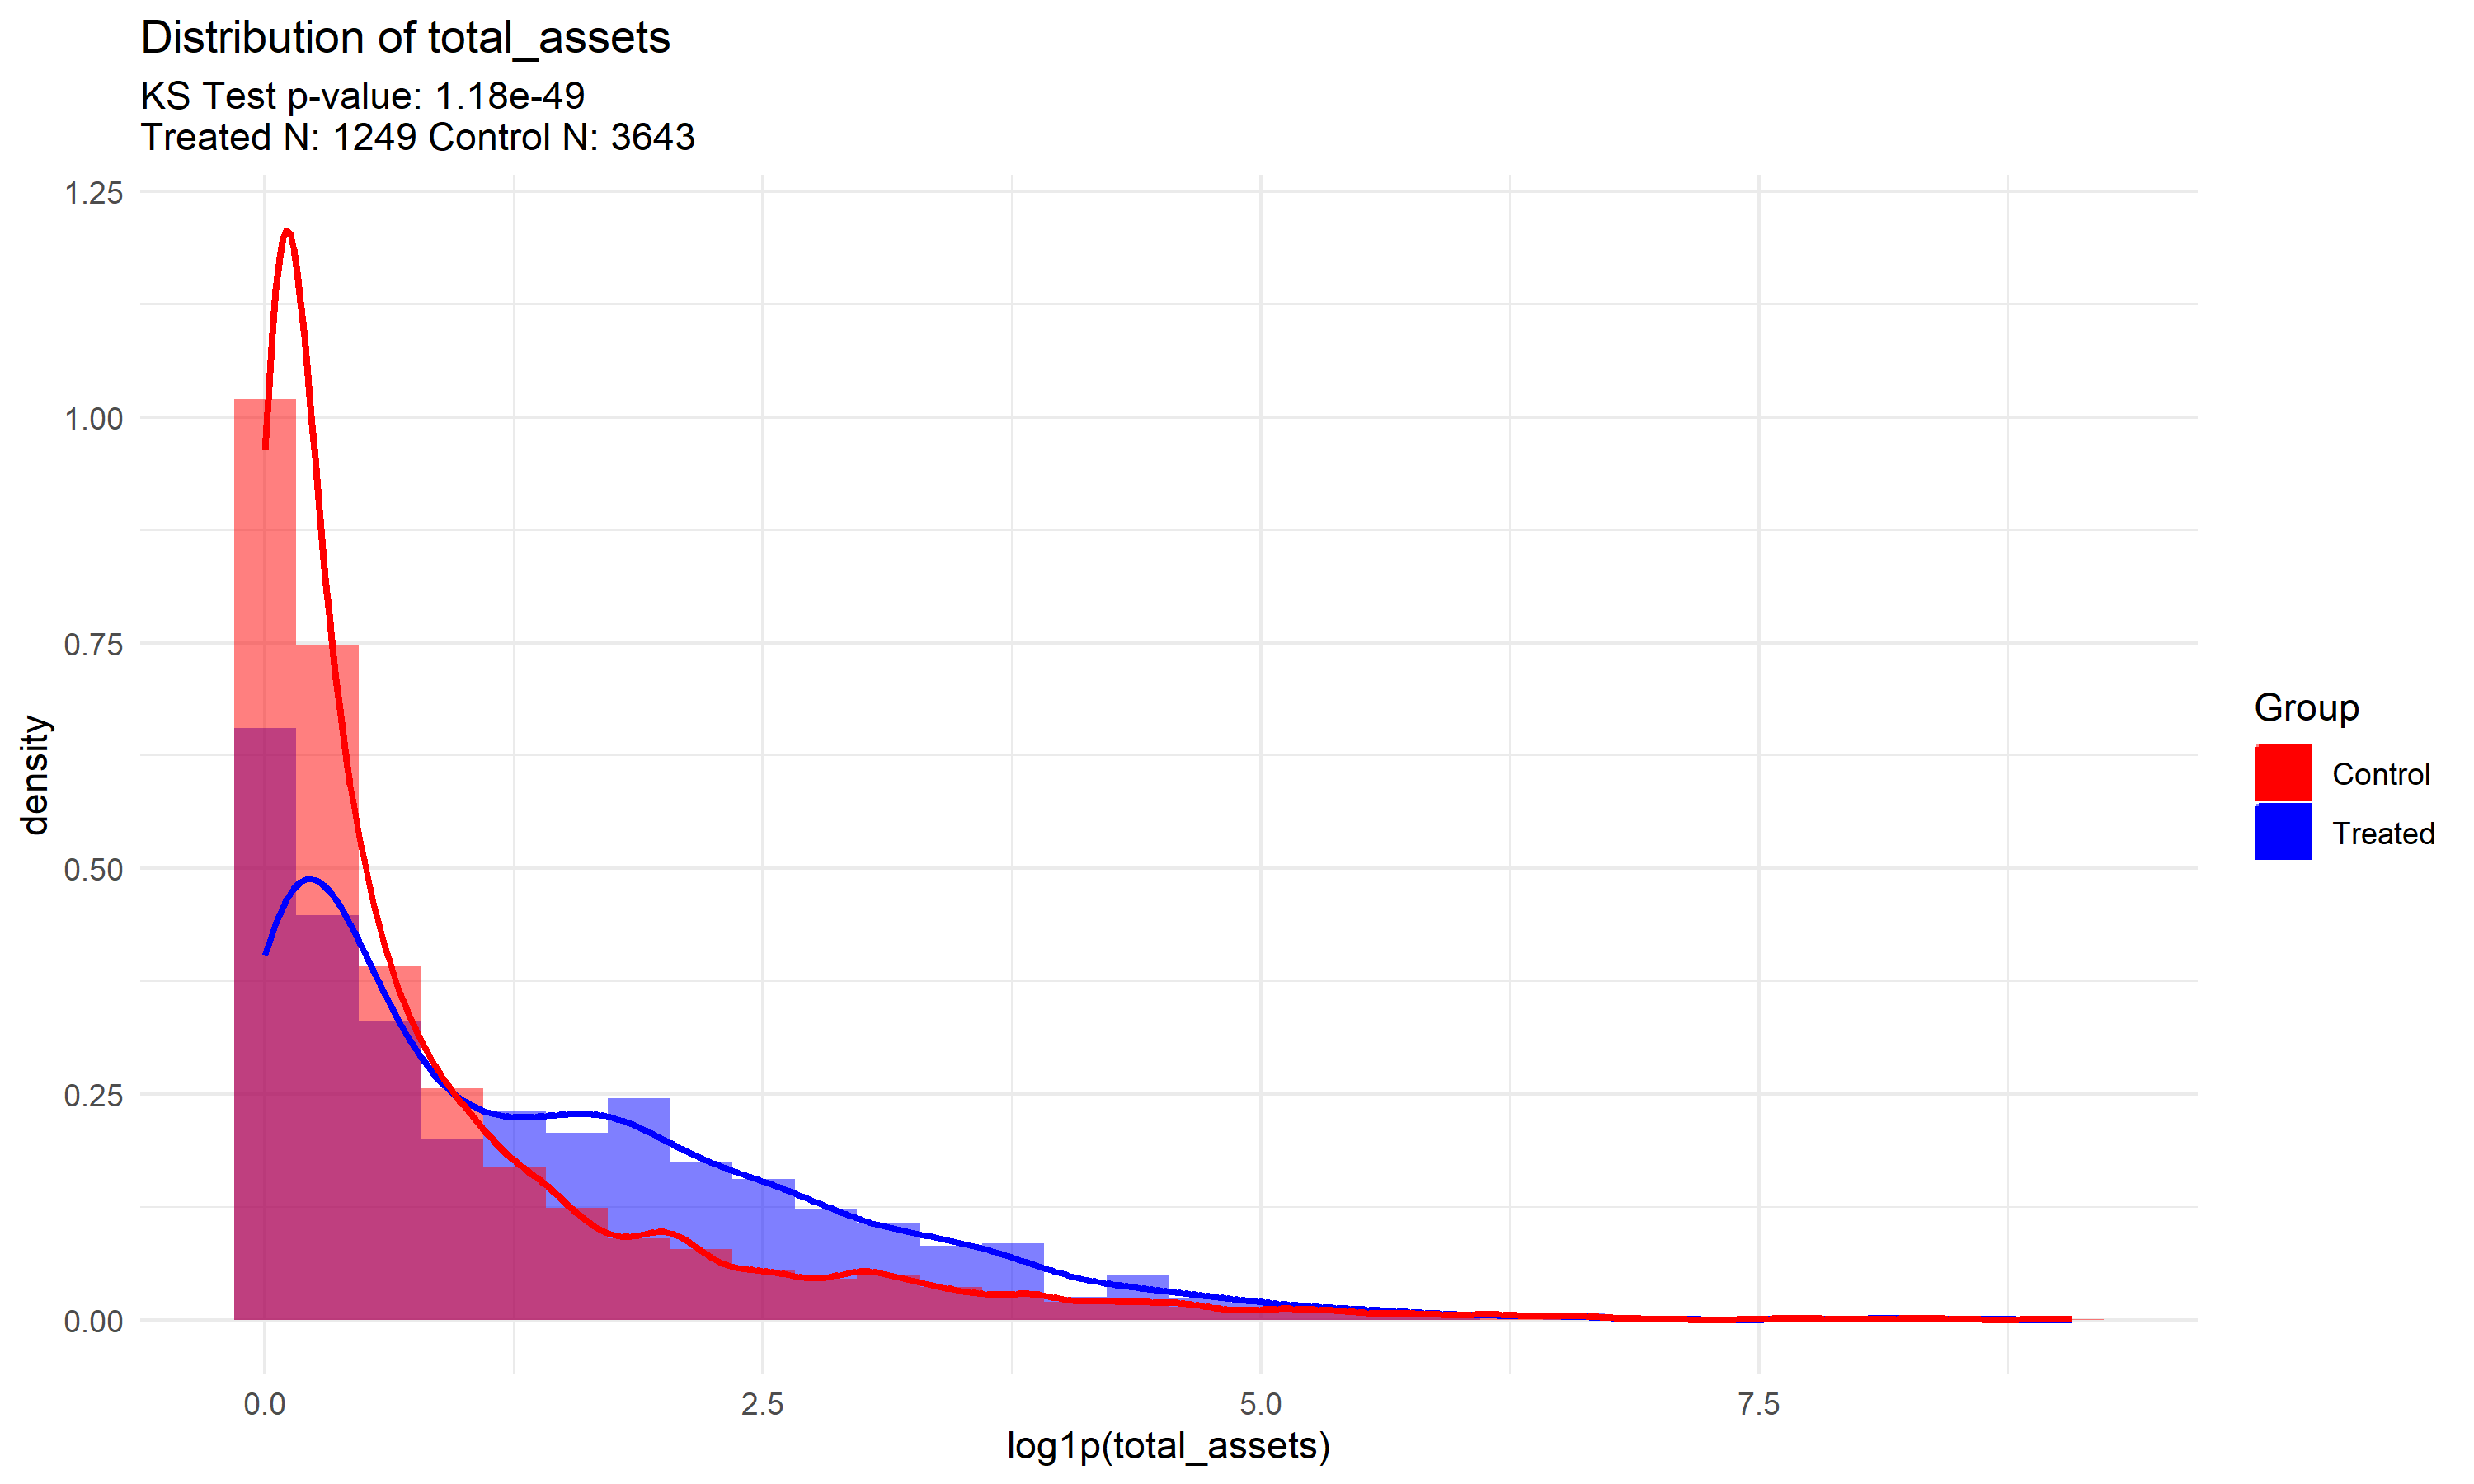
\includegraphics[width=\linewidth]{../Output/distrib_compare_total_assets_allcountries.png}
        \caption{Total Assets}
        \label{fig:total_assets}
    \end{subfigure}
    \hfill
    \begin{subfigure}[b]{0.45\textwidth}
        \centering
        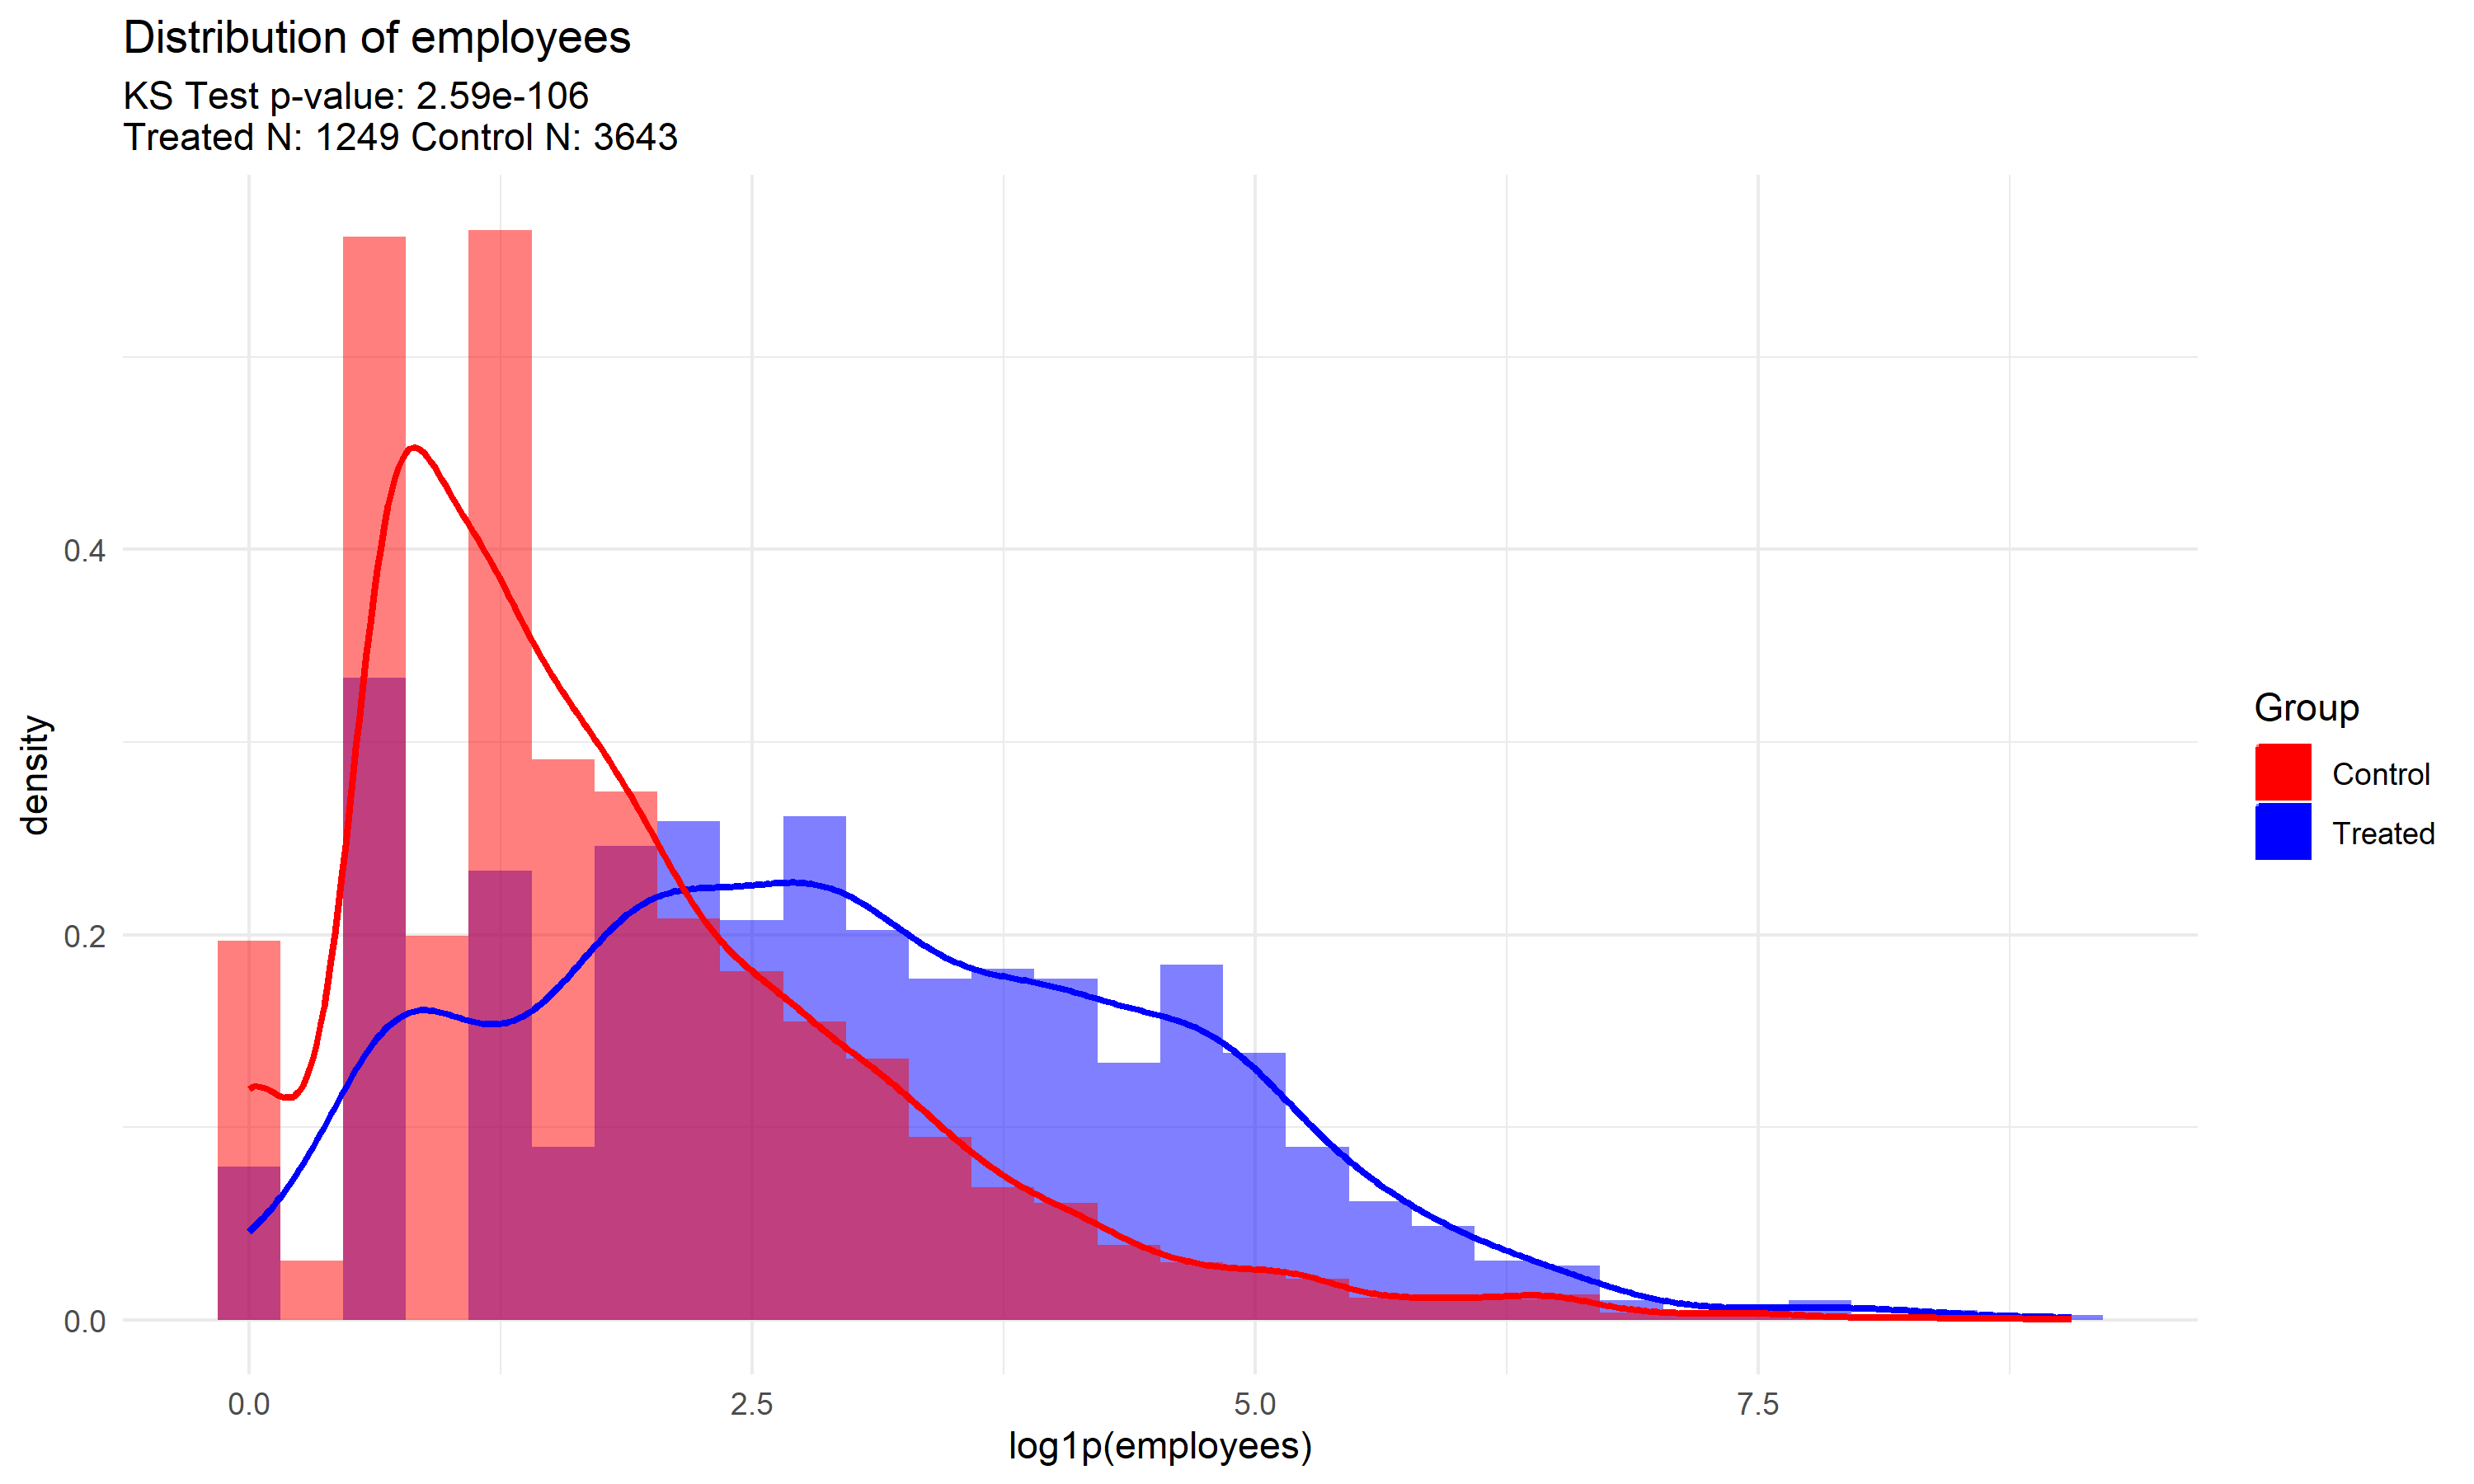
\includegraphics[width=\linewidth]{../Output/distrib_compare_employees_allcountries.png}
        \caption{Employees}
        \label{fig:employees}
    \end{subfigure}
    \vfill
    \begin{subfigure}[b]{0.45\textwidth}
        \centering
        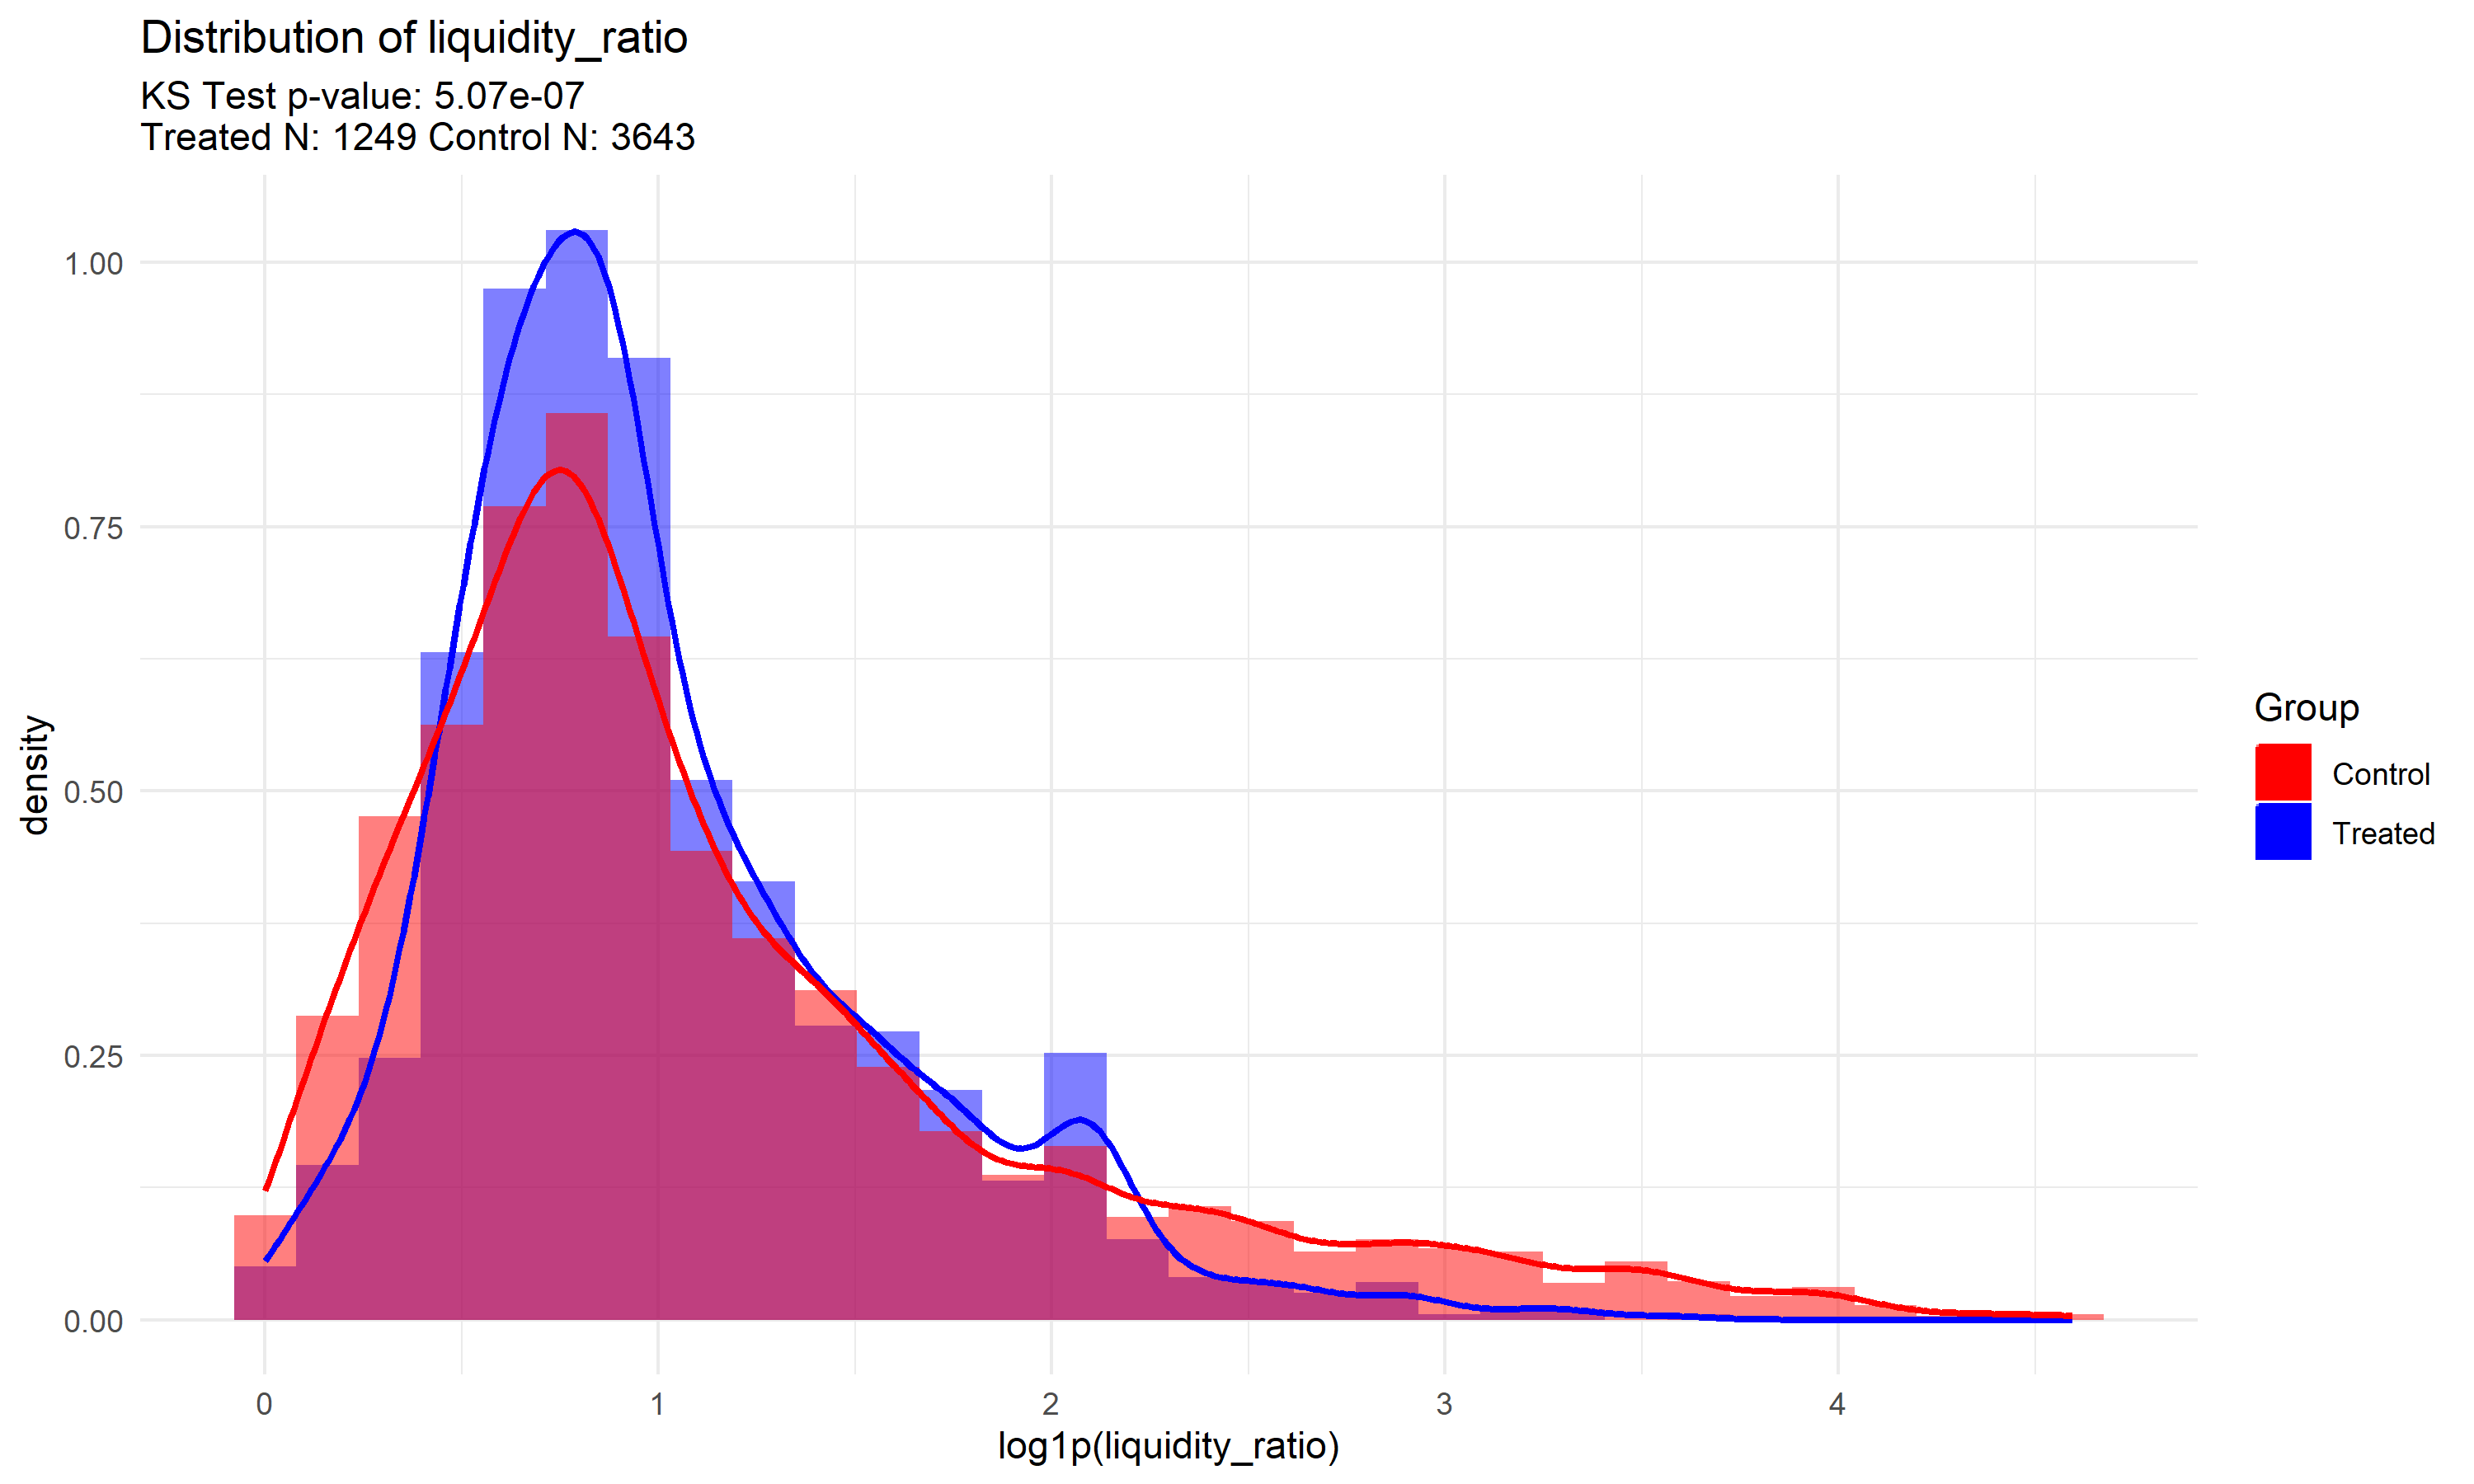
\includegraphics[width=\linewidth]{../Output/distrib_compare_liquidity_ratio_allcountries.png}
        \caption{Liquidity Ratio}
        \label{fig:liquidityratio}
    \end{subfigure}
    \hfill
    \begin{subfigure}[b]{0.45\textwidth}
        \centering
        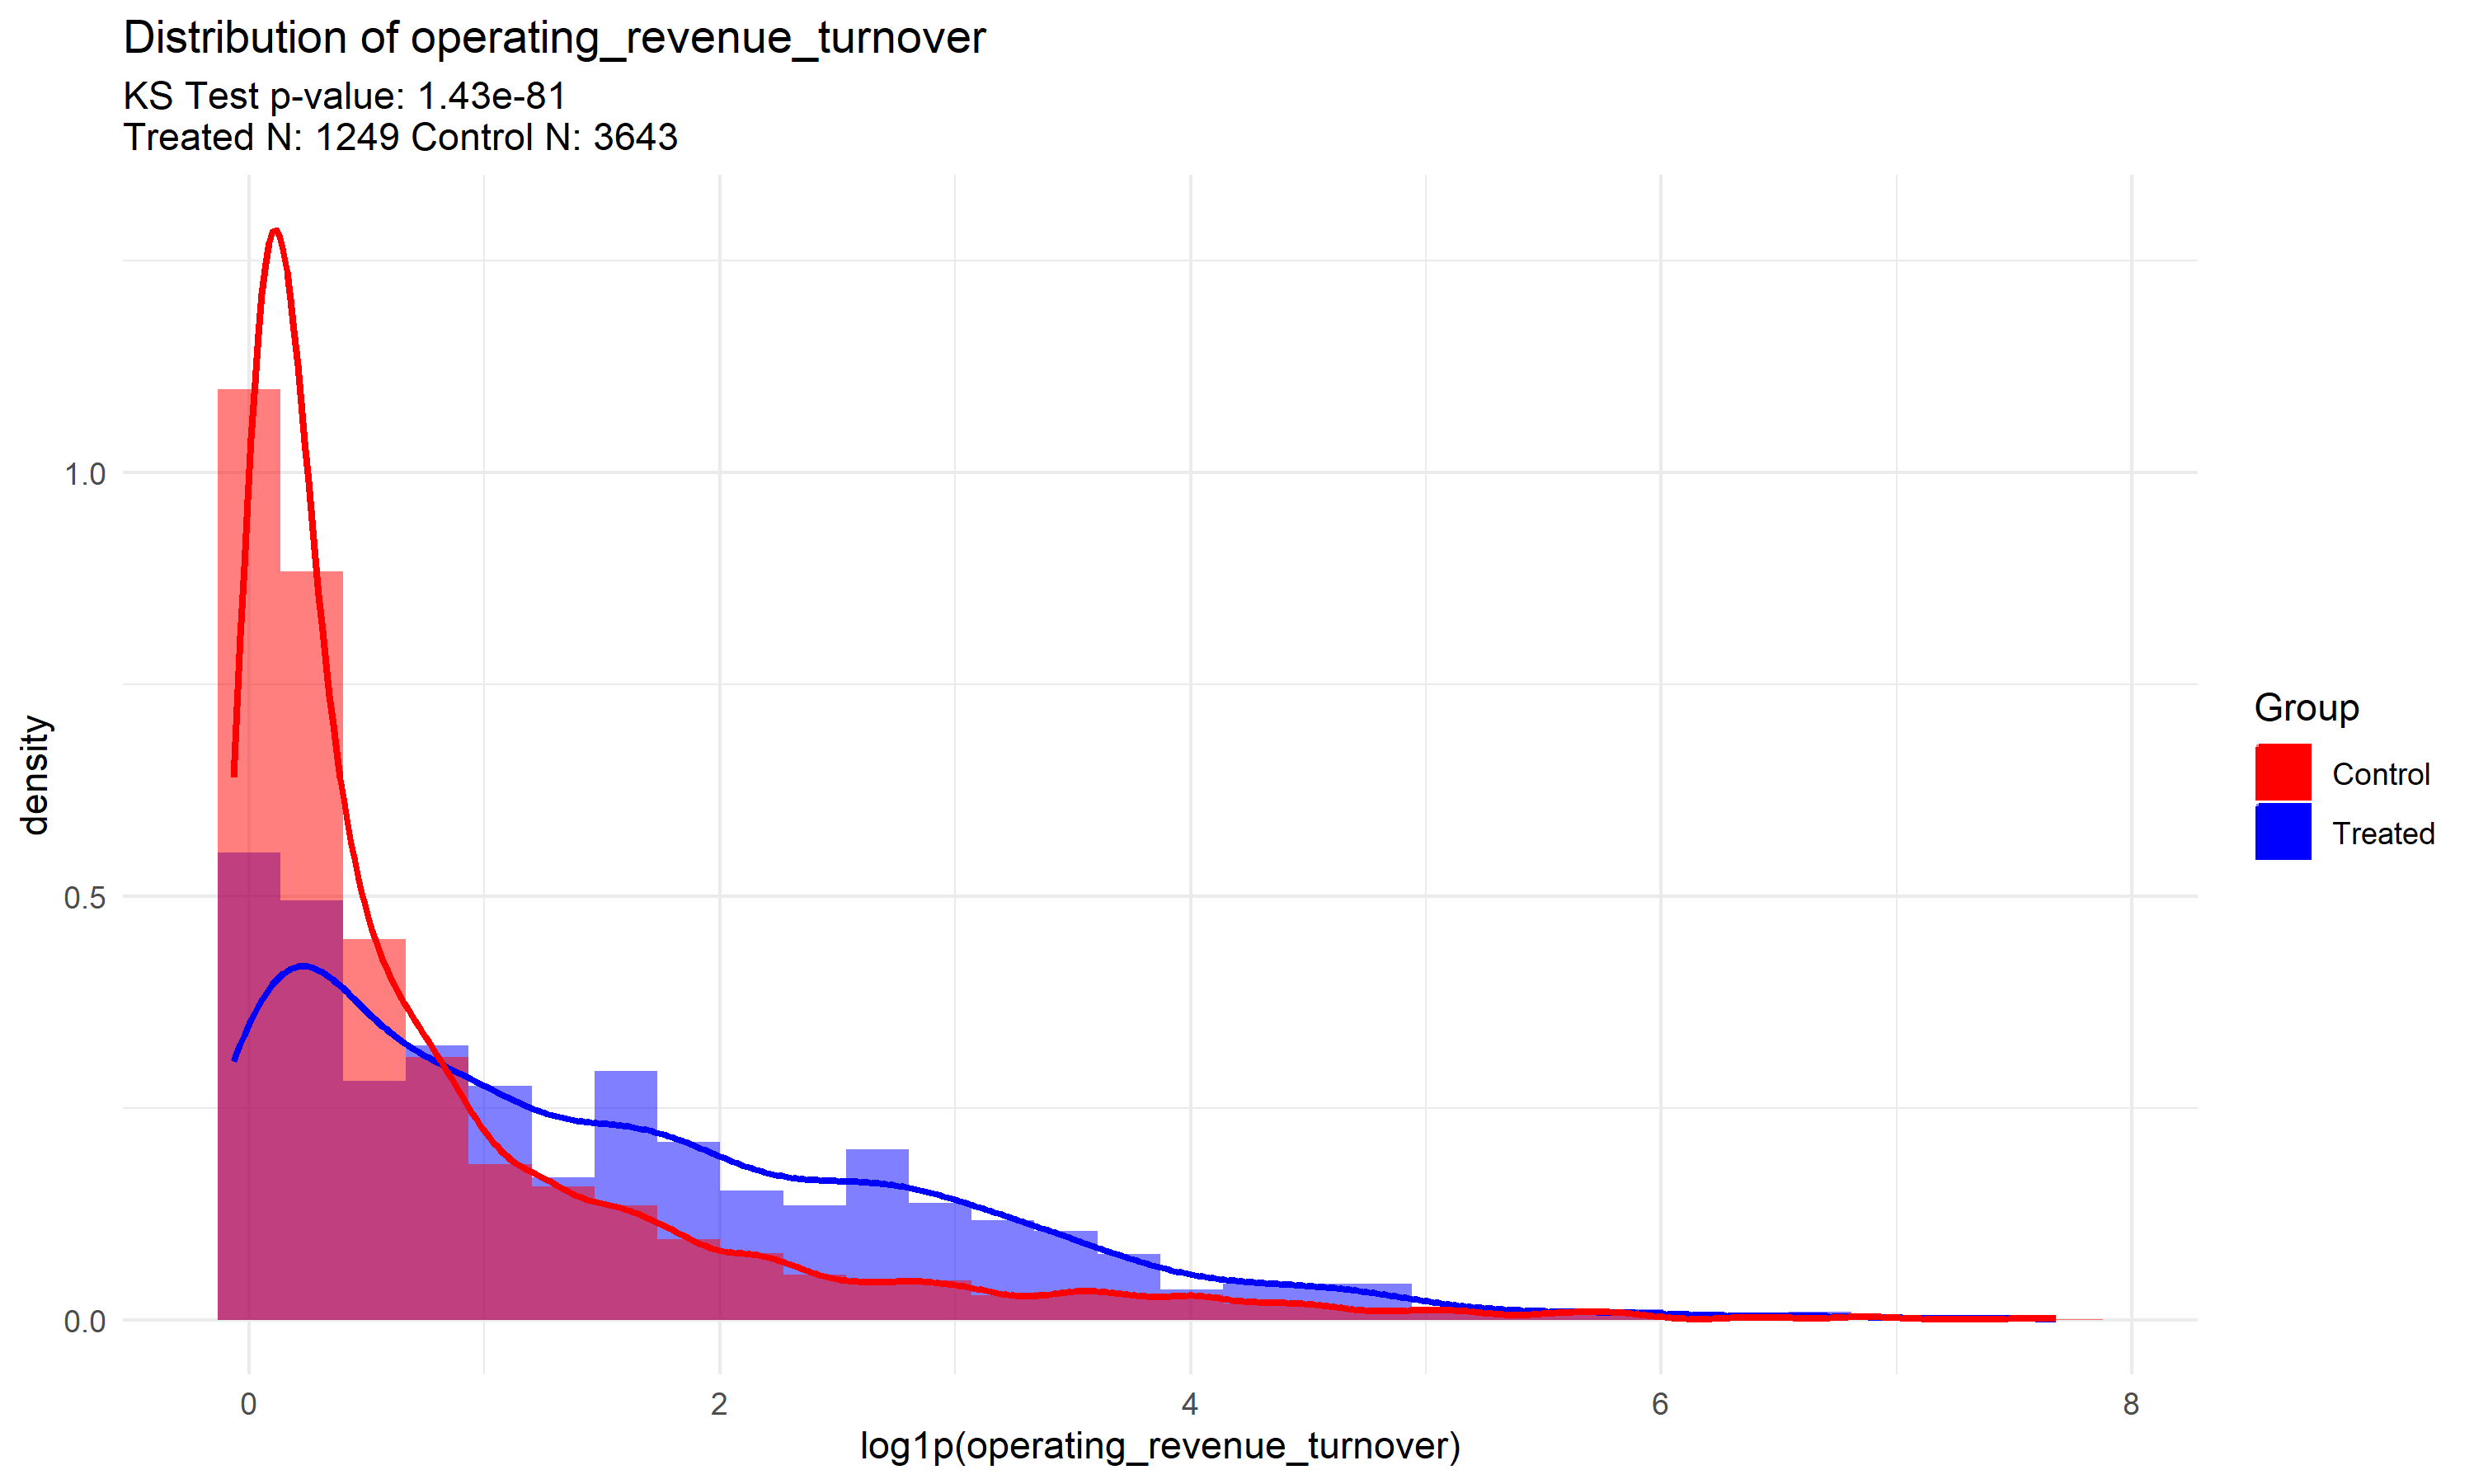
\includegraphics[width=\linewidth]{../Output/distrib_compare_operating_revenue_turnover_allcountries.png}
        \caption{Turnover}
        \label{fig:turnover}
    \end{subfigure}
    \vfill
    \begin{subfigure}[b]{0.45\textwidth}
        \centering
        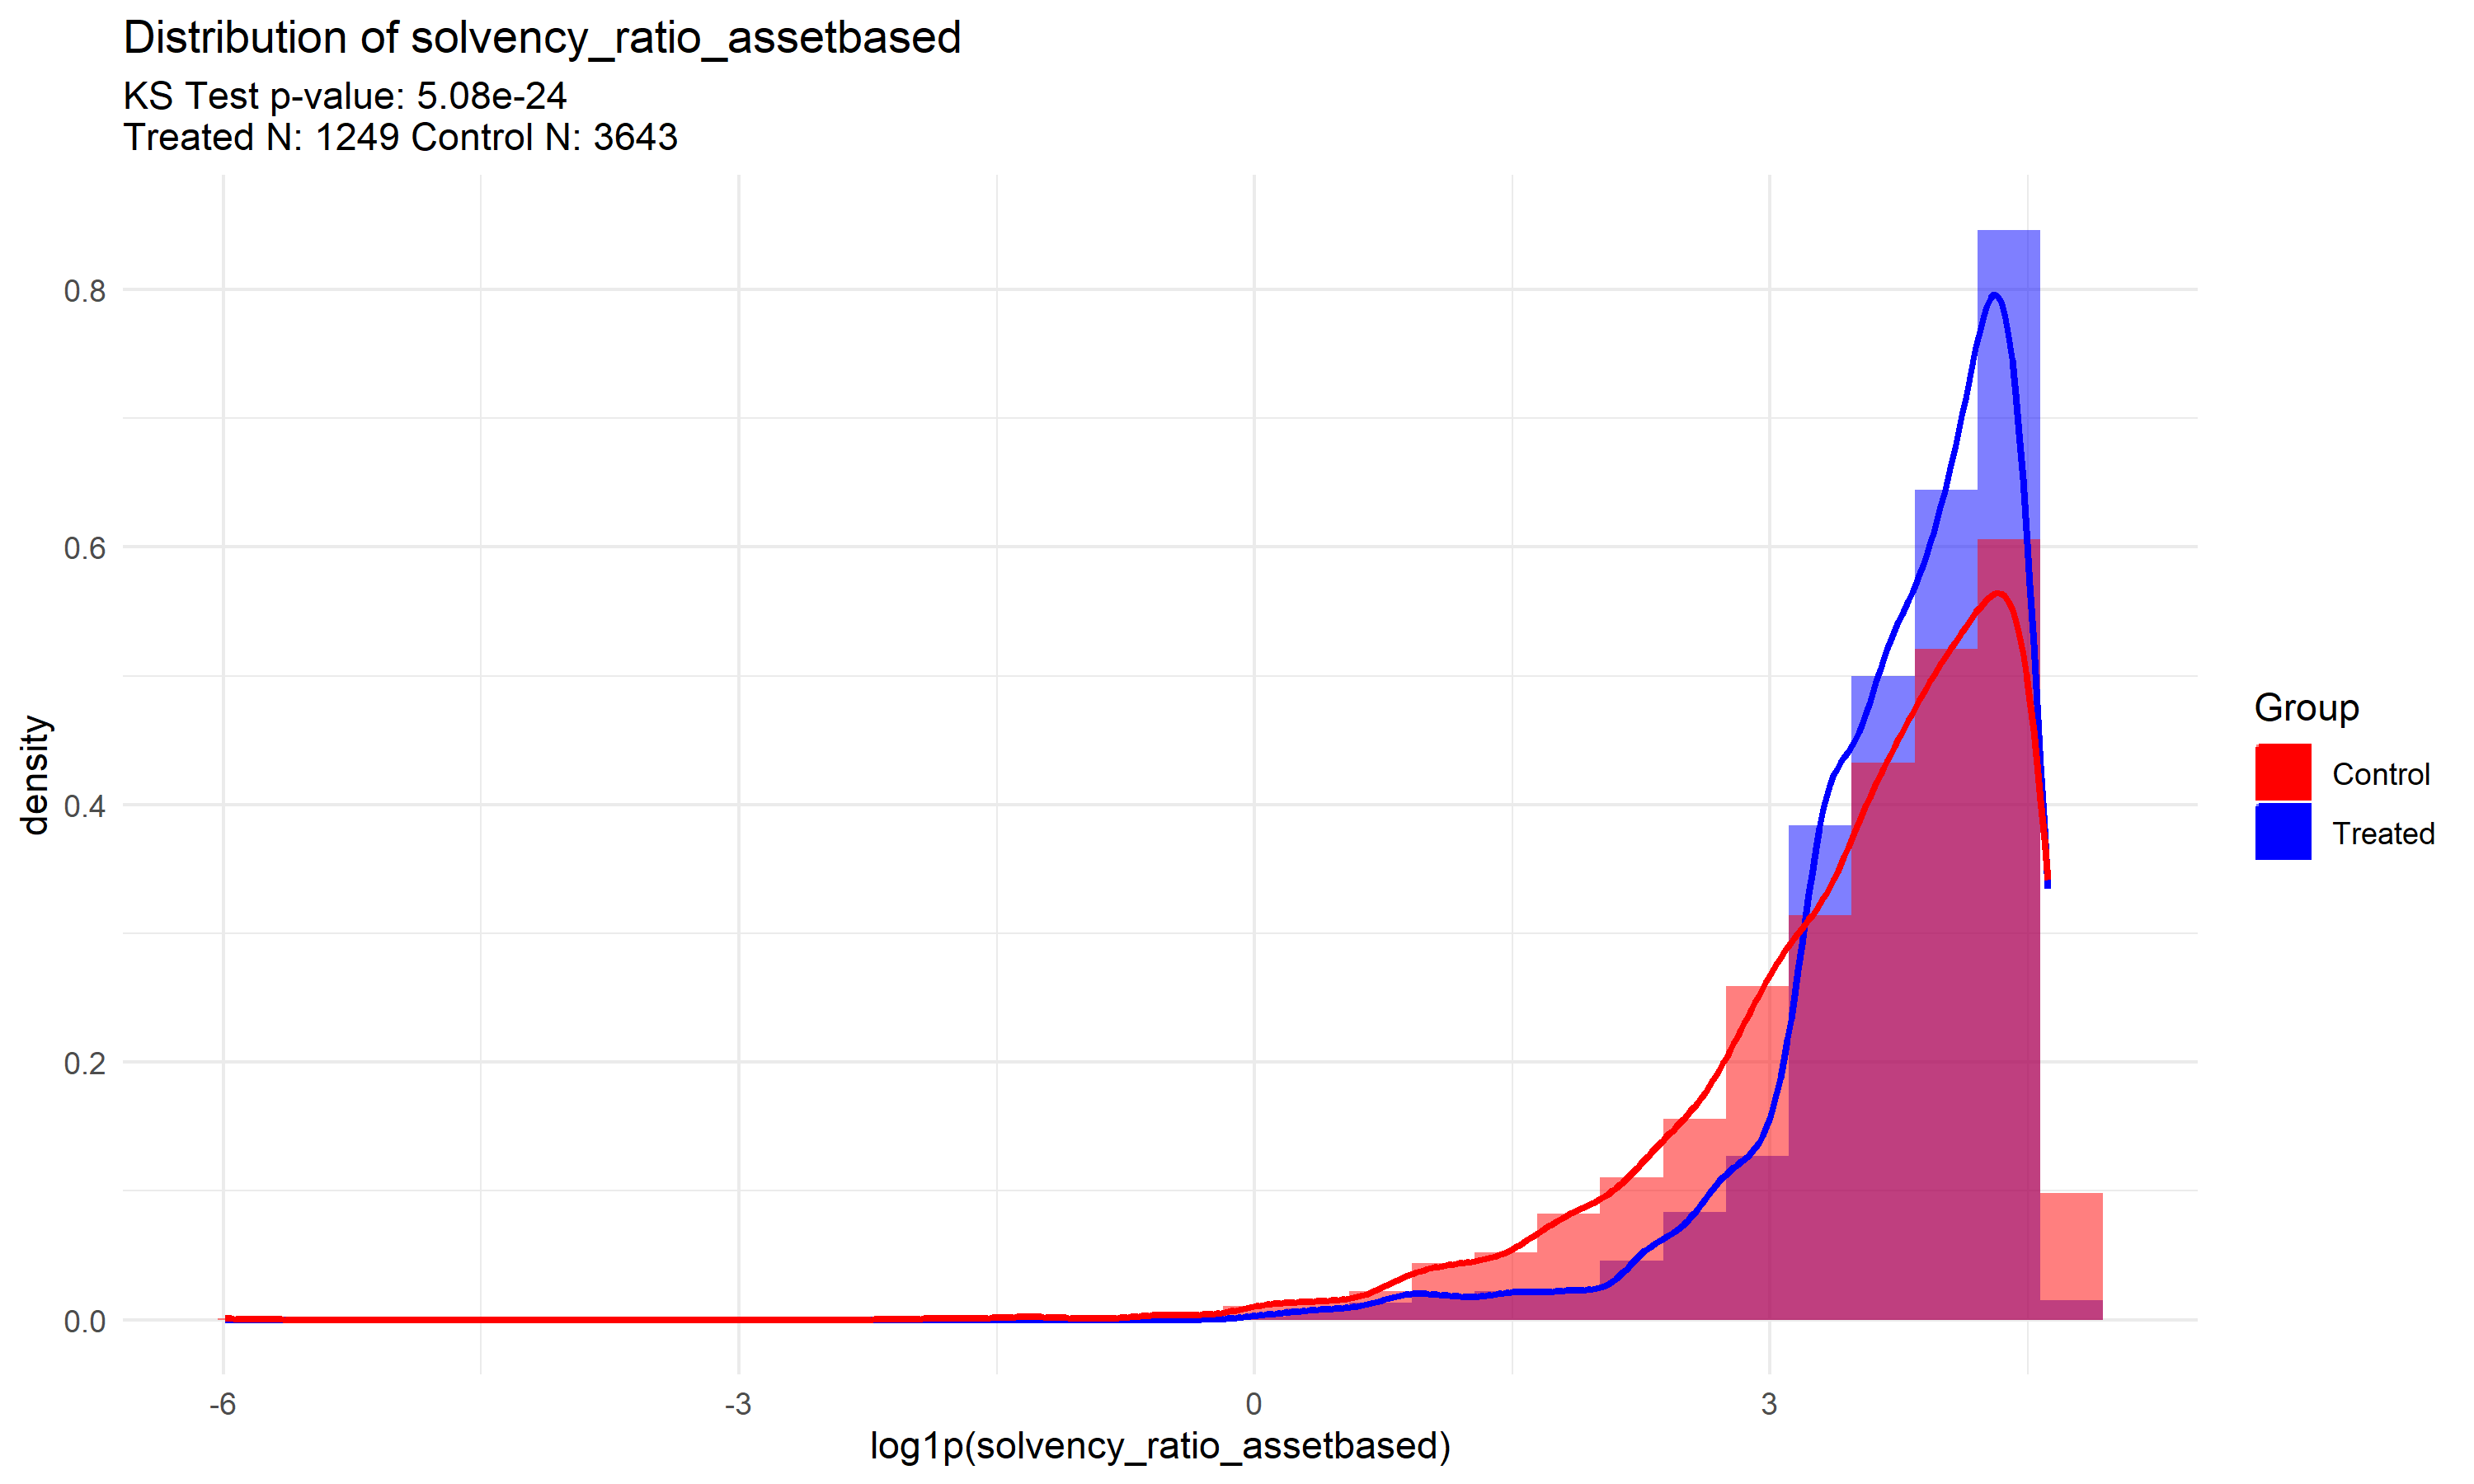
\includegraphics[width=\linewidth]{../Output/distrib_compare_solvency_ratio_assetbased_allcountries.png}
        \caption{Solvency Ratio}
        \label{fig:solvency_ratio}
    \end{subfigure}
    \caption{Distribution Comparisons Across All Countries}
    \label{fig:distribution_comparisons_lotsofvasrs}
\end{figure}

\par I also wanted to compare the sectors in which the firms operate, to see if we can find significant differences there as well. To do that, I divided the firms in the treated and control group using the NACE classification. Industry codes from NACE come as 4-digit codes, but I aggregated them to the 2-digit level to have a more general classification, as well as a more readable graph. Results can be seen in the following figure (as usual, treated firms are in blue and controls in red).

\begin{figure}[h!]
    \centering
    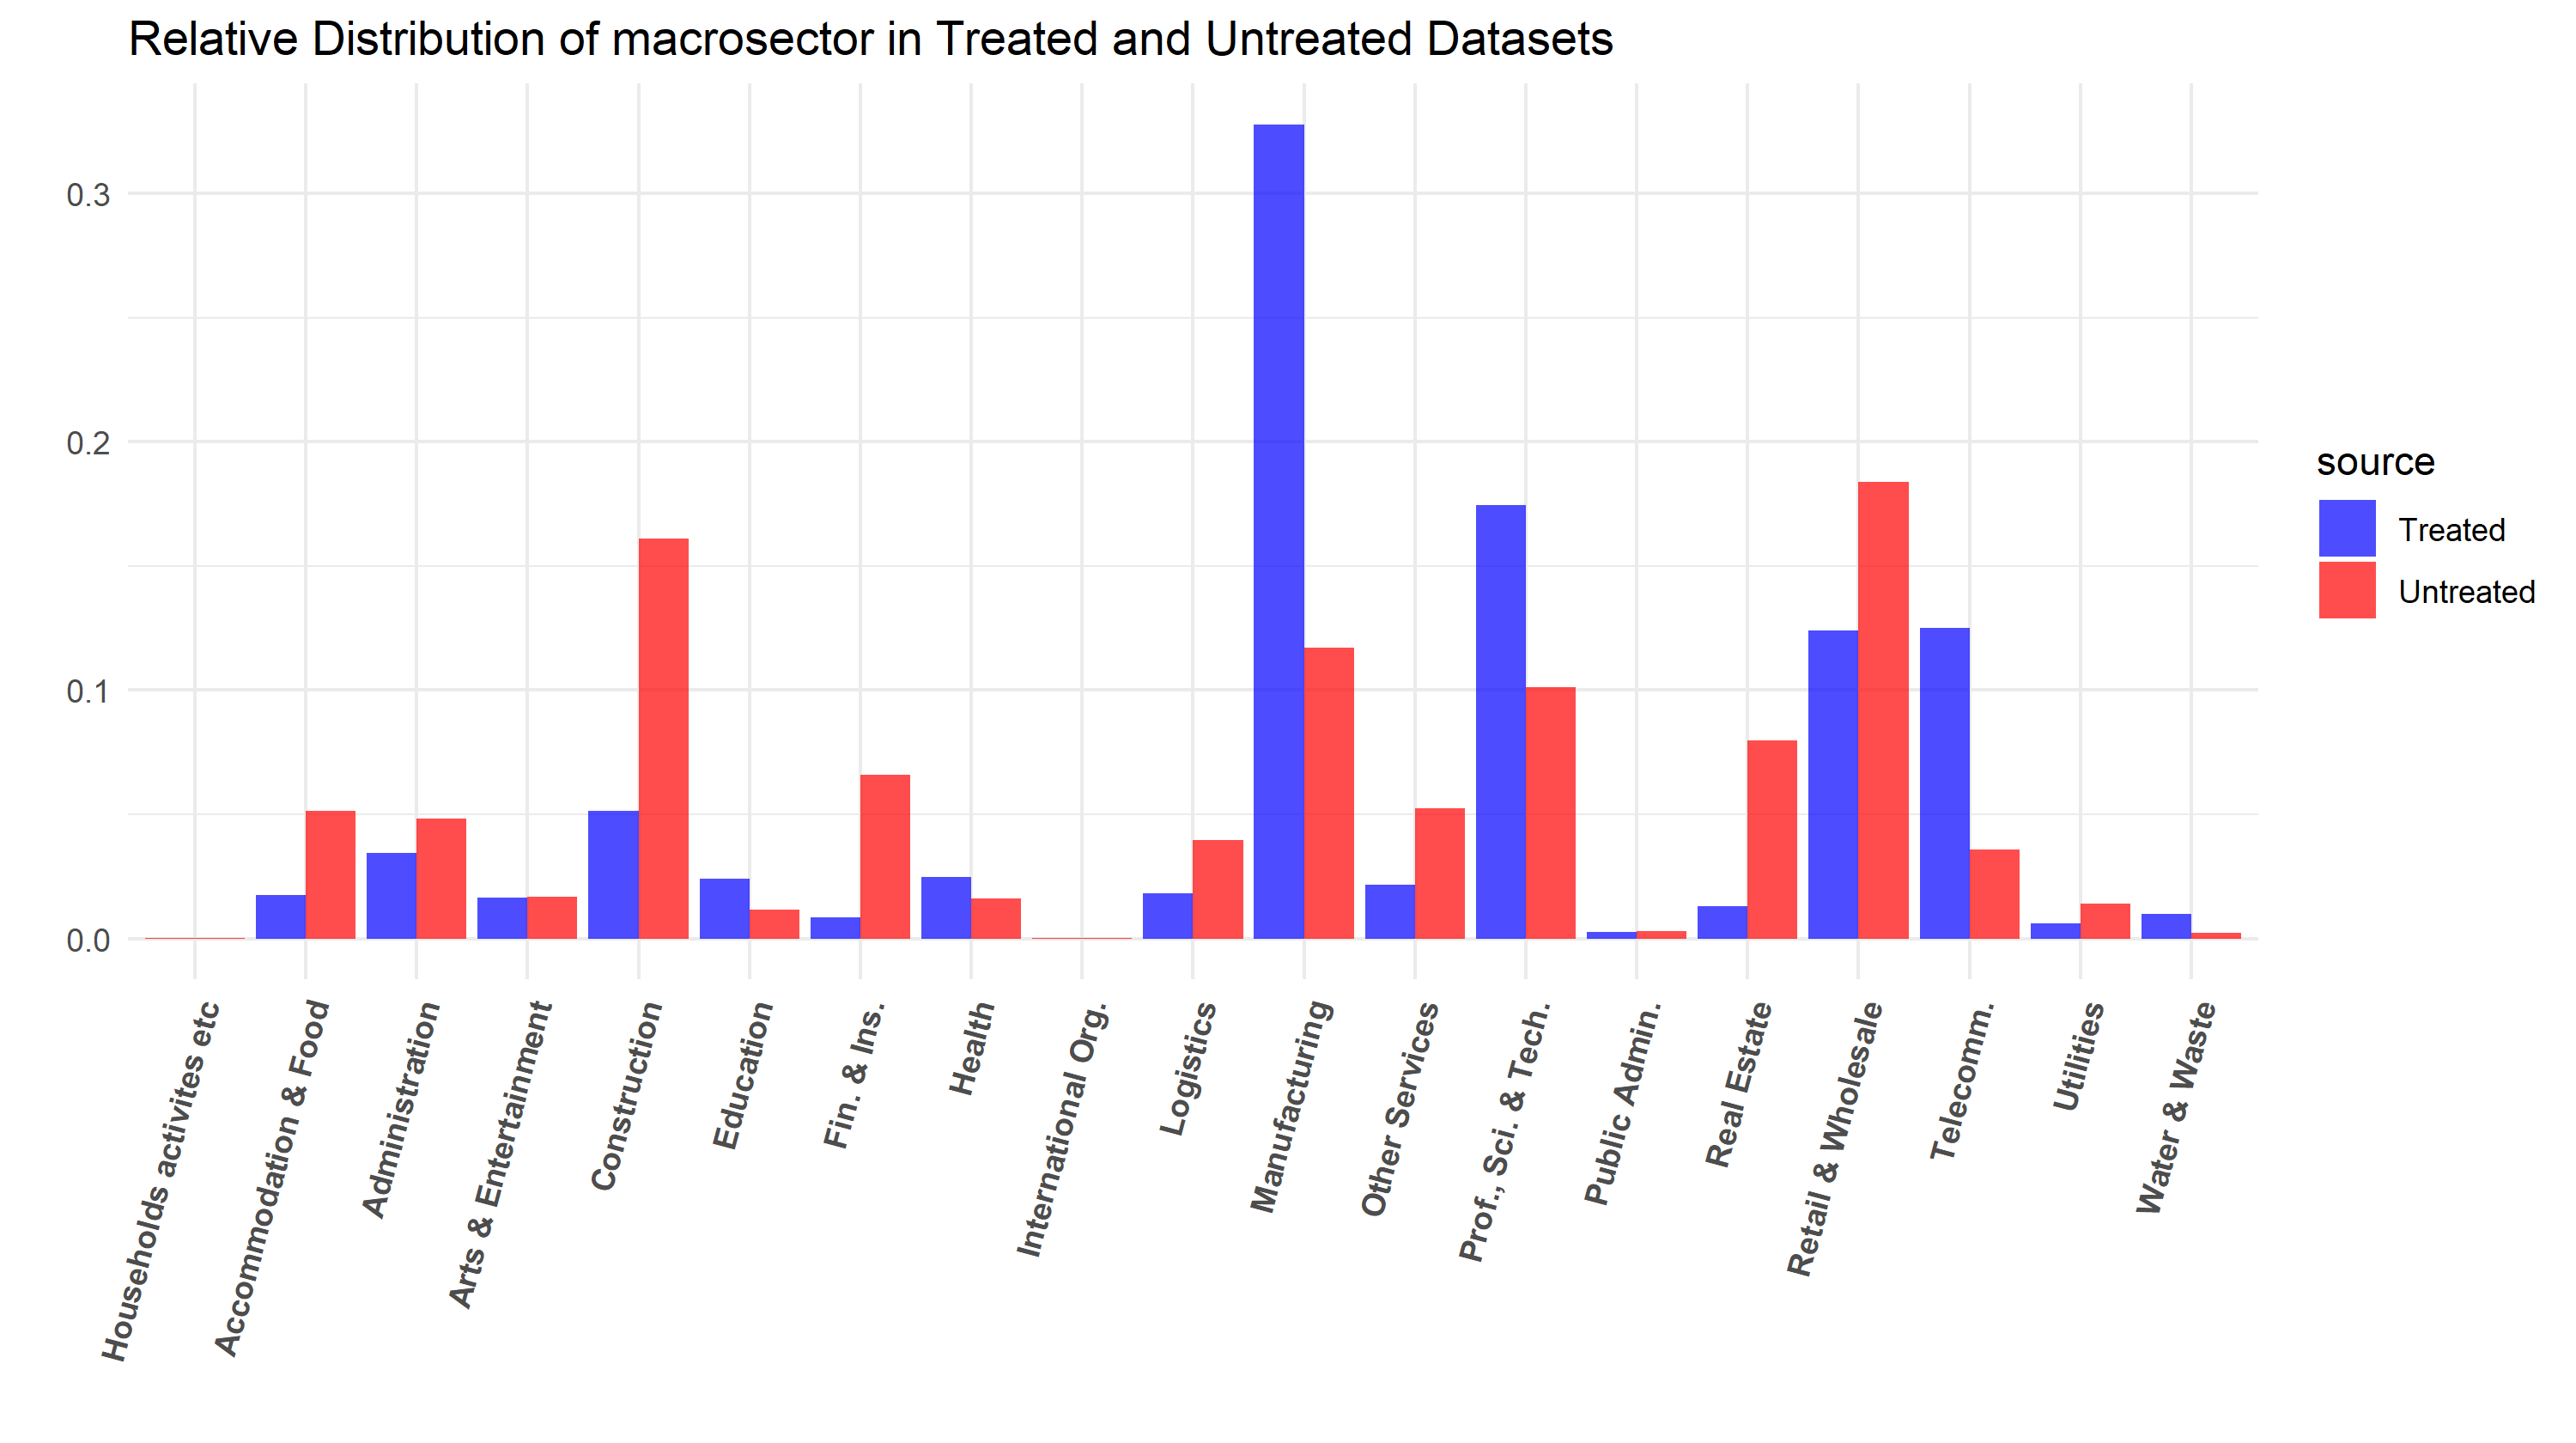
\includegraphics[width=\linewidth]{../Output/macrosectorsplot_compared.png}
    \caption{Comparison of Macro-Sectors in Treated and Control Group}
    \label{fig:distrib_compare_macrosectors_allcountries}
\end{figure}

\par What is immediately noticeable from the graph is how much the sectoral distribution of firms differs between treated and controls. In particular, the macrosectors relating to "Manufacturing", "Professional, scientific and technical activities" and "Information and communication" are overrepresented in the treated group, while "Real estate", "Construction" and "Wholesale and retail trade" are underrepresented.
\par This is probably due to the declared focus of the EDIH initiative on digitalization, and especially on manufacturing technologies. After all, a manufacturing firm can be more easily interested in digitalization since it can profit more from the adoption of these new technologies, while a construction firm may not be as interested. This is an argument for including the macrosector as an independent variable in the regression.

\section{Geocoding, distance and density computation}

\par As I was mentioning in the introductory section of this chapter, I wanted to investigate the effect of the distance of firms from the closest EDIH hub on the probability of participation in the program. 
\par At the start of the process, what I had were addresses, either taken from the DMA survey (for the treated sample) or from the ORBIS database (for the control sample)\footnote{In a small number of cases, ORBIS reported coordinate information as well as the address; in those cases, I took those as being correct, and did not run those observations through the geocoding process}.
\par To get the correct coordinates of the firms, I used the \texttt{geocode} function (part of the \texttt{tidygeocoder} package) in R. This function takes the address string as input and runs the Nominatim API to get coordinate information from the OpenStreetMap database. The function is efficient, but the Nominatim API limits requests to one per second, so I had to time 1 second of sleep for the code for it to work properly. Thus, the process was time-consuming\footnote{Note that the process was done for roughly 18000 firms in the control group, as well as all the firms in the DMA databse, and every EDIH in the database as well. Thus, the geocoding part of the process took some hours to complete}.

\par Once the geocoding loop was done, I had the coordinates of all the firms in the treated and control groups. You can see their geographical distribution in the following map, where treated firms are represented by the red dots, control firms by the light blue dots, and EDIH hubs by the dark blue and dark green dots (the former for EU-financed hubs, the latter for Seal of Excellence hubs).

\begin{figure}[h!]
    \centering
    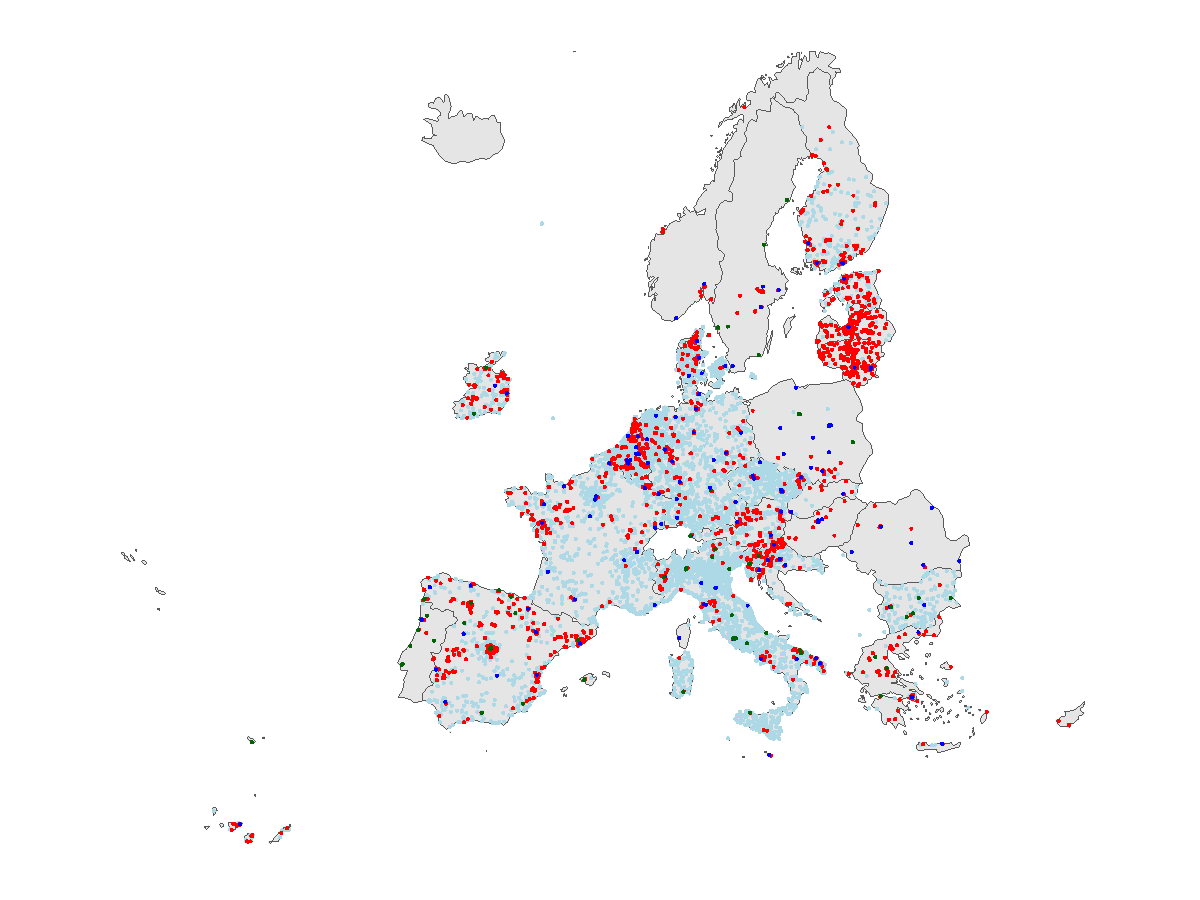
\includegraphics[width=\linewidth,trim={2.8cm 0cm 2.5cm 0.5cm},clip]{../Output/EU_map.pdf}
    \caption{\centering{Map showing the geographical distribution of treated firms (in red), control firms (in light blue) and EDIH hubs (with EU-funded ones in dark blue and regionally/nationally funded ones in dark green) in the whole EU}}
    \label{fig:map_obs_EU}
\end{figure}

\par Already from this map of the whole EU, we can notice some aspects of the analysis we've already discussed. For example, it is clear how the ORBIS coverage is not equally good in each EU country. As a reference, look at the difference in coverage between France and Belgium, or between Italy and Spain. This is important to keep in mind when designing the regression model to use for the analysis, and this is on of the reasons why we will include the country-groups' dummies as an independent variable in the regression.

\par One other thing that we can notice is how the EDIH coverage is not uniform across EU countries, and not even across regions in the same country. For example, let's take a look in detail at Italy, reported individually in the map below.

\begin{figure}[h!]
    \centering
    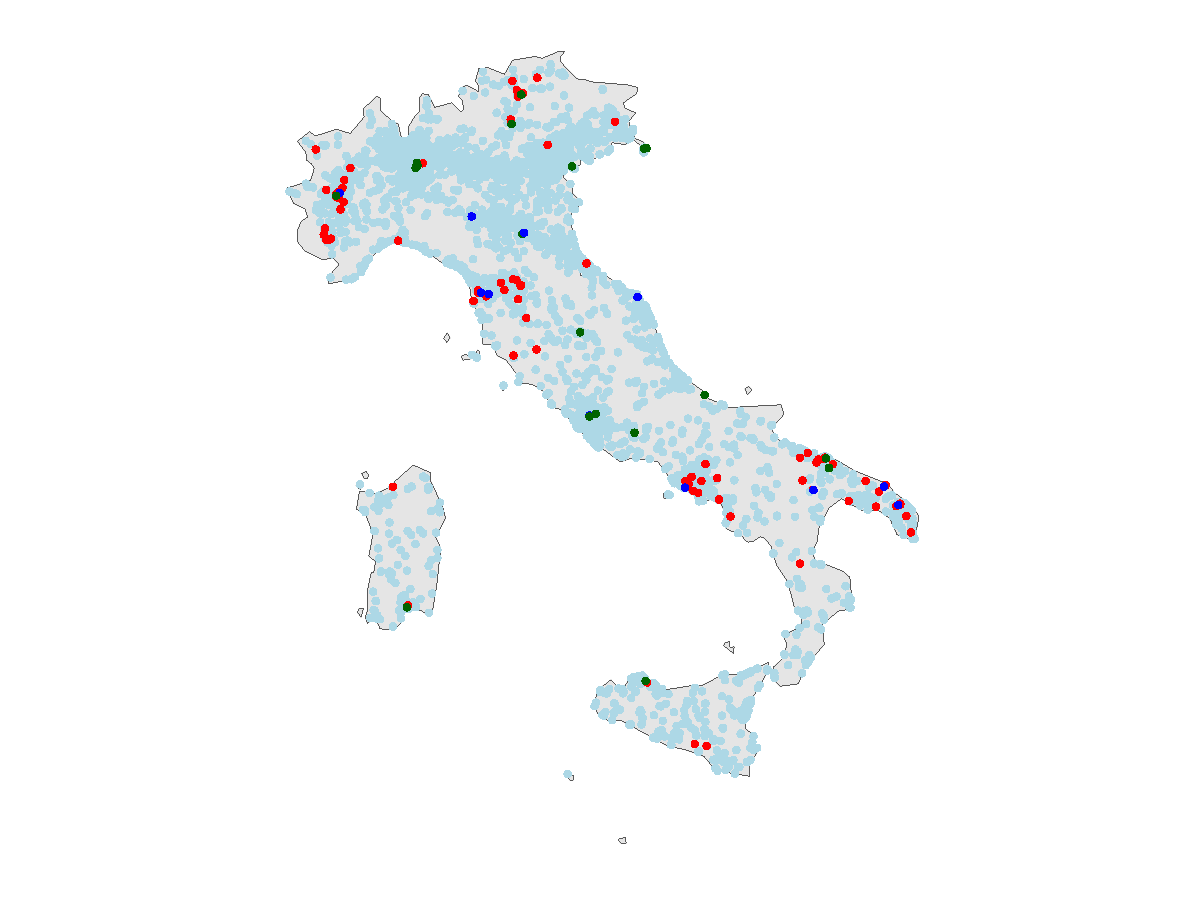
\includegraphics[width=\linewidth]{../Output/IT_map.pdf}
    \caption{\centering{Map showing the geographical distribution of treated firms (in red), control firms (in light blue) and EDIH hubs (with EU-funded ones in dark blue and regionally/nationally funded ones in dark green)} in Italy. All the other individual countries' maps are reported in the Appendix.}
    \label{fig:map_obs_IT}
\end{figure}

\par From this map of firms in Italy, we can see how treated firms are concentrated close to the location of EDIH offices\footnote{One additional note can be made about the fact that EU-financed EDIHs seem to have more treated firms around them w.r.t Seal of Excellence Hubs, which are instead financed through national or regional funds. This fact is not valid only in Italy, and can be an avenue for future research on the effectiveness of the initiative itself. Initial data from the DMA seems in fact to suggest that EU-EDIHs are more active than SoEs. However, please note that this is more likely to be due to a lack of certainty about funding, which is likely delaying start of opeerations for SoEs. Time will tell if their performance will be better in the future.}. This is an initial indication of the negative effect of distance on the probability of accessing the initiative.

\par However, it can also be noted that in many cases treated firms are concentrated in clusters around densely "populated" areas, where also hubs tend to be located. Thus, without including a measure of the "firm density" of the territory in which the firms operate, the effect of proximity to the hubs is likely to get confounded by the effect of being in an area of high firm density\footnote{We can think of firm density as impacting the decision of the firm to participate in the EDIH initiative in many mays. For example, it can be that being surrounded by many firms exposes the firm more to competition, thus making it more imperative to digitalize, and thus seeking help to do so.}.


\par Now that we have coordinates for every firm and EDIH, computing distances is a straightforward (albeit lengthy) process. To get distances, for every firm in the database of treated and controls, I computed its distance with each of the EDIHs in the database, and then chose the closest one. This was done using the \texttt{distHaversine} function from the \texttt{geosphere} package in R. This function takes the 2 sets of coordinates as input and computes the distance between them using the Haversine formula, which is the most accurate way to compute distances on a sphere. 

\par After having computed the distances, I then computed the firm density for each firm. To do this, I utilized the following procedure. For every firm, I first computed the distance between it and every other firm in the database (both treated and controls). Then, I filtered out all firms more distant than a certain threshold\footnote{After a few trials, I settled on a threshold of 5 km, deemed as a good compromise to have an acceptable level of variance in firm density. In fact, a threshold too high would have led to a very high density for every firm, while a threshold too low would have led to a very low density for every firm.}, and counted the number of firms left. You can see a representation of the process in the following figure.

\begin{figure}[ht]
    \centering
    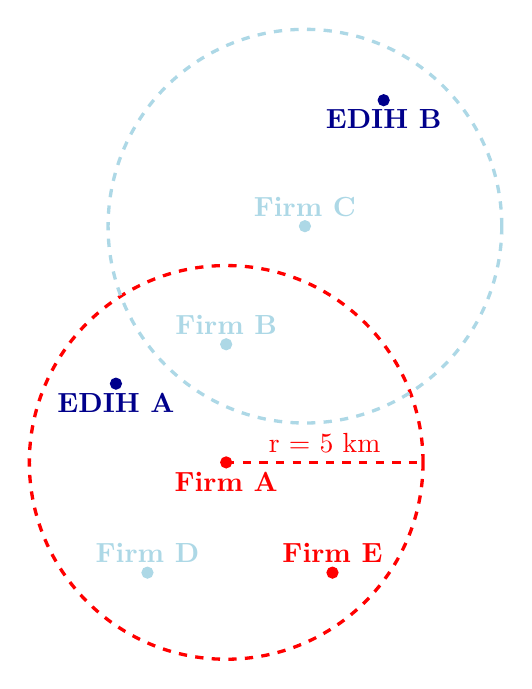
\begin{tikzpicture}
        % Draw a horizontal segmented line to represent the radius
        \draw[red, thick, dashed] (0,0) -- (2.5,0) node[midway, above] {r = 5 km};

        % Draw firms as dots
        \filldraw[red] (0,0) circle (2pt) node[anchor=north] {\textbf{Firm A}};
        \filldraw[lightblue] (0,1.5) circle (2pt) node[anchor=south] {\textbf{Firm B}};
        \filldraw[lightblue] (1,3) circle (2pt) node[anchor=south] {\textbf{Firm C}};
        \filldraw[darkblue] (-1.4,1) circle (2pt) node[anchor=north] {\textbf{EDIH A}};
        \filldraw[darkblue] (2,4.6) circle (2pt) node[anchor=north] {\textbf{EDIH B}};
        \filldraw[lightblue] (-1,-1.4) circle (2pt) node[anchor=south] {\textbf{Firm D}};
        \filldraw[red] (1.35,-1.4) circle (2pt) node[anchor=south] {\textbf{Firm E}};
        
        % Draw a circle around the firms to represent density
        \draw[red, very thick, dashed] (0,0) circle (2.5cm);

        \draw[lightblue, very thick, dashed] (1,3) circle (2.5cm);
    \end{tikzpicture}
    \caption{\centering{Diagram showing the criteria for computing firm density. In the image, Firm A has a firm density of 3, while Firm C has a firm density of 1.}}
    \label{fig:firm_density_glyph}
\end{figure}

\par In the diagram you can see how Firm A has a firm density of 3, as firms B, D, and E all fall inside of the 5km-radius circle around Firm A (while EDIH offices are not counted as firms). On the other hand, Firm C has a firm density of only 1, since Firm B is the only one inside the 5km-radius circle around Firm C (and again, EDIH offices are not counted as firms). From the diagram you can also see how in the computation of firm density, both treated and control firms are taken into account.

\par Thus, the designed measure of firm density can be considered as an accurate proxy of the density of firms on the EU territory, at least when the ORBIS bias is taken into account.

\par Now that we have computed both firm distance and density measures, we can add them to the initial treated-control comparison, to see how they differ between the two groups, as seen in the following tables.




\begin{figure}[ht]
    \centering
    \begin{subfigure}[b]{0.45\textwidth}
        \centering
        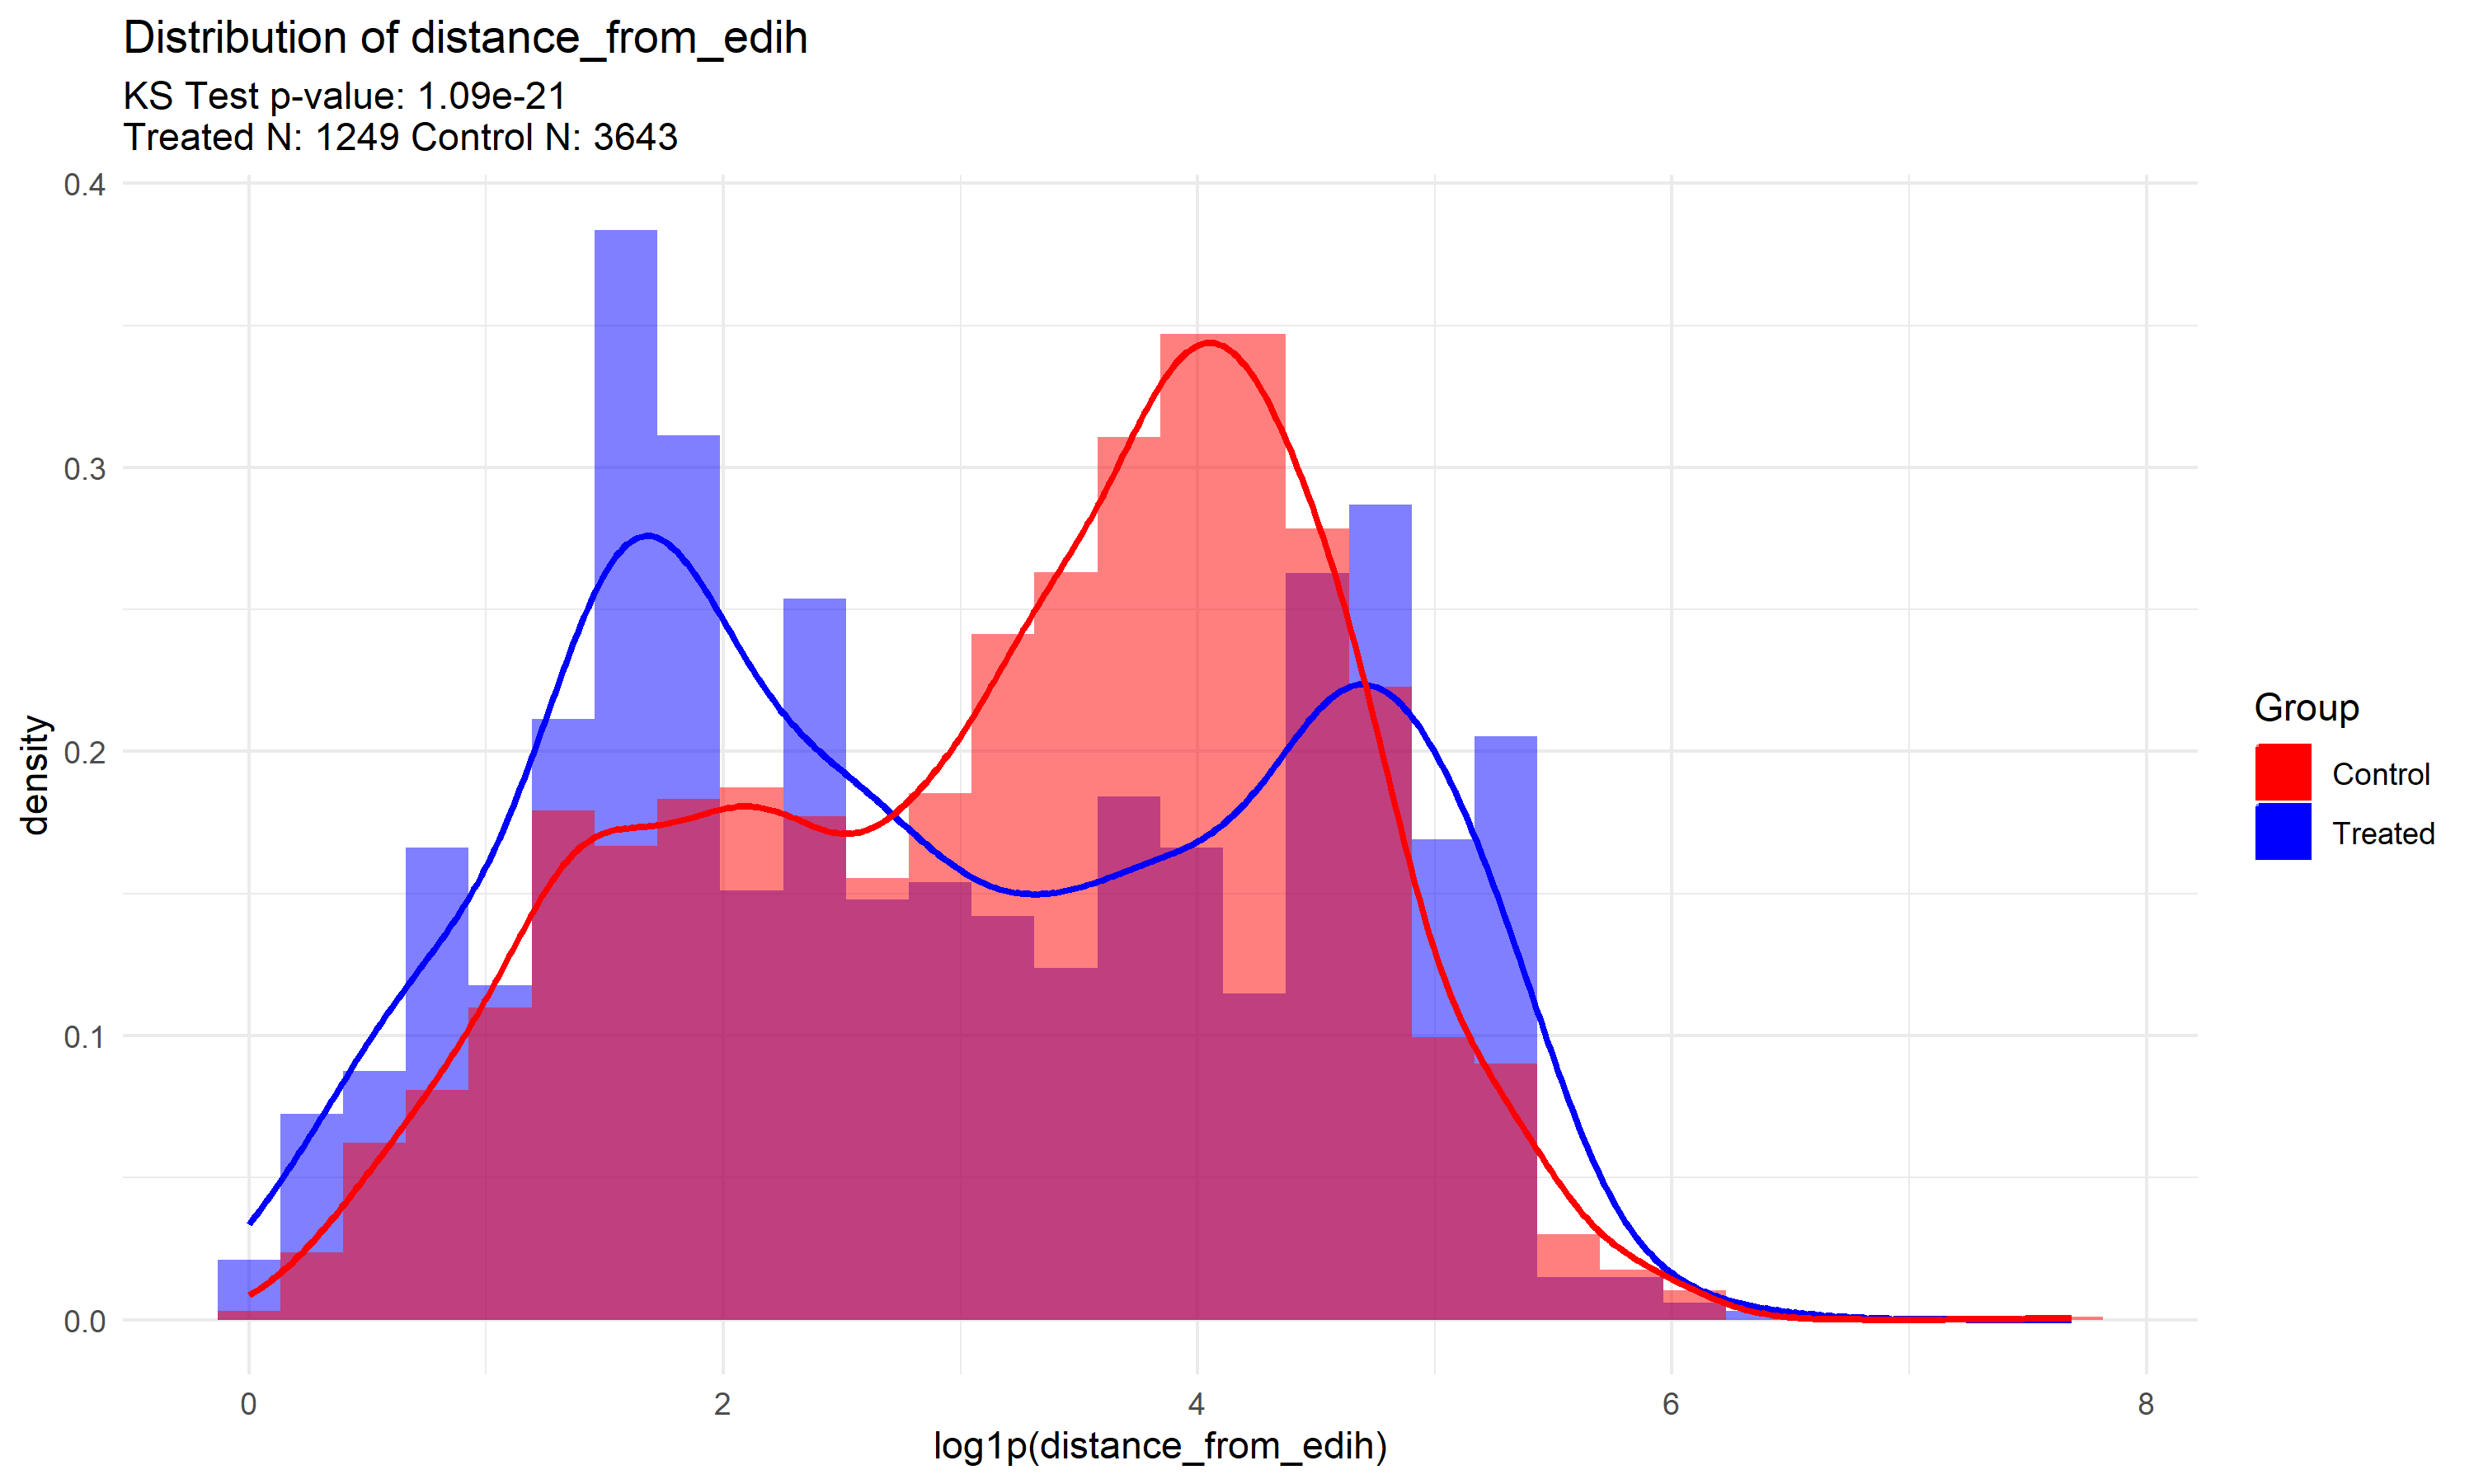
\includegraphics[width=\linewidth]{../Output/distrib_compare_distance_from_edih_allcountries.png}
        \caption{Distance from closest EDIH}
        \label{fig:distance_from_edih}
    \end{subfigure}
    \hfill
    \begin{subfigure}[b]{0.45\textwidth}
        \centering
        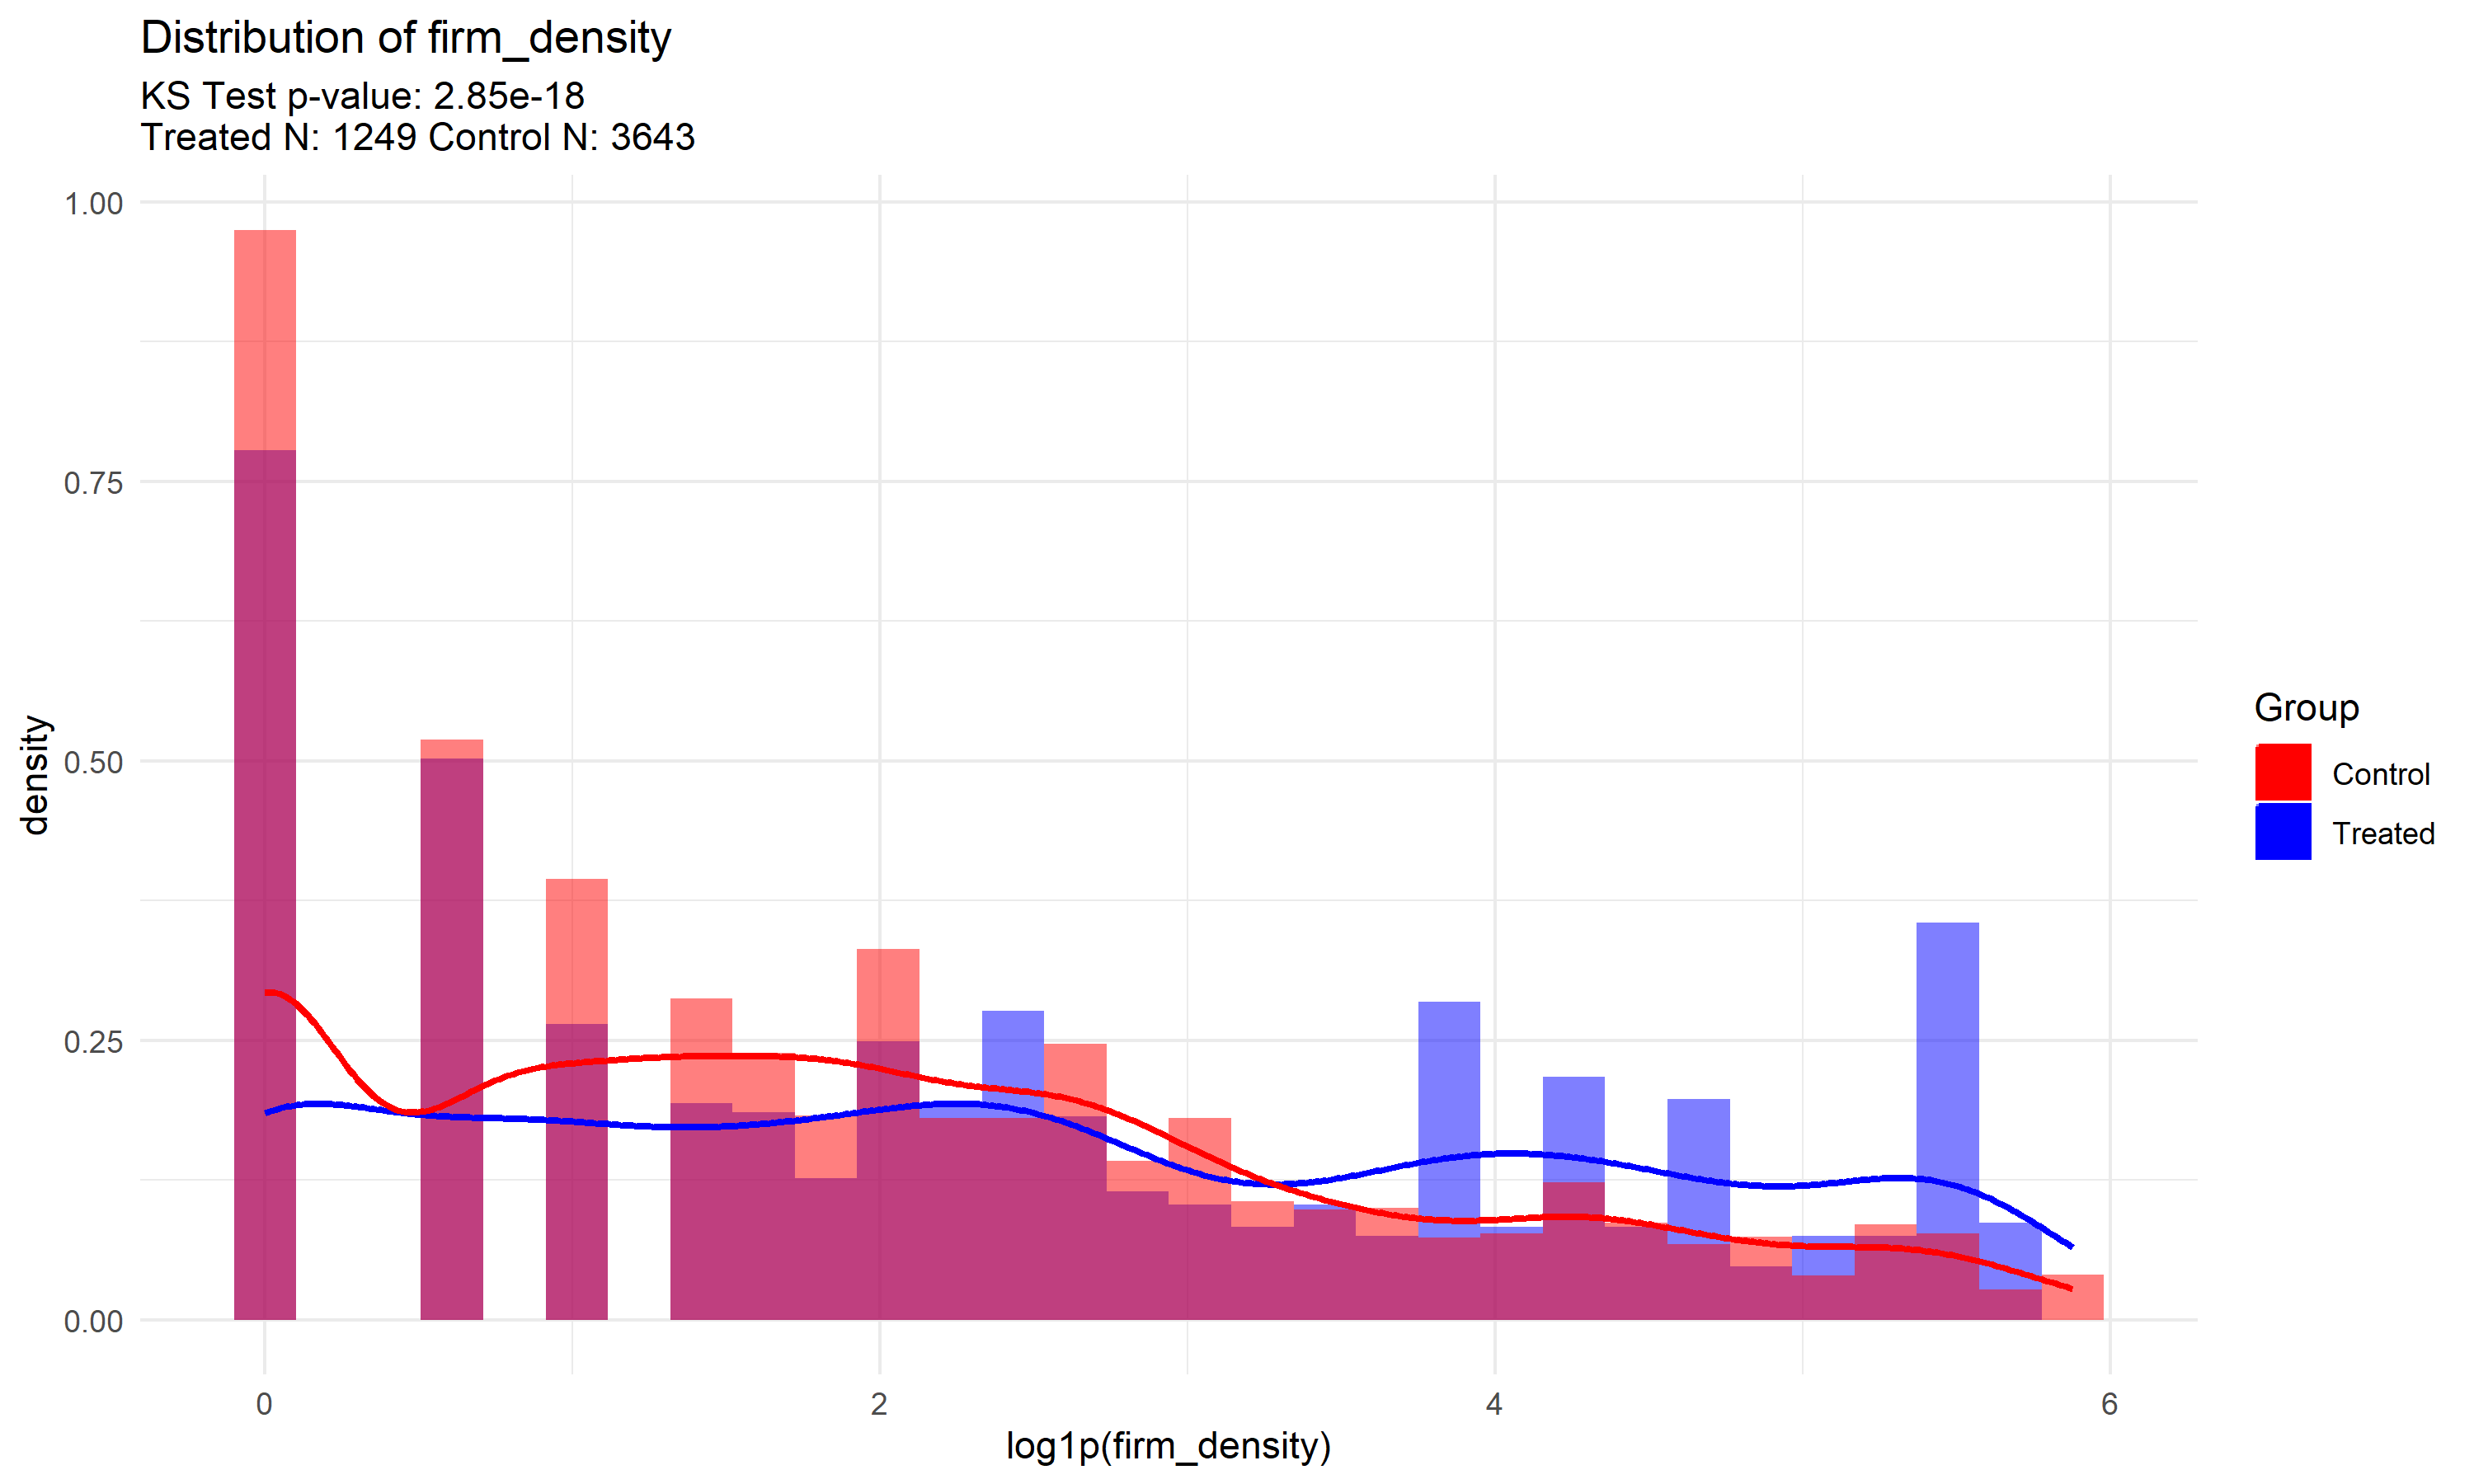
\includegraphics[width=\linewidth]{../Output/distrib_compare_firm_density_allcountries.png}
        \caption{Firm Density}
        \label{fig:firm_density}
    \end{subfigure}
    \caption{Distribution Comparisons of distance and firm density across all Countries}
    \label{fig:distribution_comparisons}
\end{figure}

\par In both cases, we can see from the results of the KS-tests that the treated and control groups hail from different distributions. In addition, it seems that treated firms are on average closer to the EDIH hubs, are also located in areas with higher firm density. This is an additional indication that the spatial dimension is significant in understanding the drivers of firms' participation to the EDIH initiative.





\section{Regression Model and Results}

\par As previously mentioned in the sections above, to analyze the drivers of participation in the EDIH initiative, I have run a probit regression model. The model includes various firm-level characteristics as independent variables, and the dependent variable is a dummy variable indicating whether the firm participated in the EDIH initiative. The model is specified as follows:

\begin{equation}
    \begin{split}
        D_{i}(\text{Treated}_{i} = 1) = \beta_{0} &+ \beta_{1} \text{Distance}_{i} + \beta_{2} \text{Firm Density}_{i} \\
        &+ \beta_{3} \text{Sector}_{i} + \beta_{4} \text{Tech Level}_{i} \\
        &+ \beta_{5} \text{Turnover}_{i} + \beta_{6} \text{Employees}_{i} \\
        &+ \beta_{7} \text{Liquidity Ratio}_{i} + \beta_{8} \text{Solvency Ratio}_{i} \\
        &+ \beta_{9} \text{Country Group}_{i} + \varepsilon_{i}
    \end{split}
\end{equation}


\par Where the dependent variable is a dummy indicating participation to the program, Distance and Firm Density are defined as above, Sector is a variable indicating the type of sector to which the firm belongs (either Manufacturing, Services or Other, with the baseline being Other). Tech Level is a variable indicating the level of technological intensity of the sector in which the firm is operating, according to the OECD taxonomy defined in \cite{oecdclassification}; in this case, the baseline is represented by the lowest level of the OECD taxonomy. Turnover, Employees, Liquidity Ratio and Solvency Ratio are all firm-level variables coming from the ORBIS database. More specifically, turnover serves as a proxy for firm profitability, employees proxies for firm size (total assets was excluded to being too collinear with employees), while liquidity ratio and solvency ratio are proxies for the financial wellbeing of the firm. Country Group is a dummy indicating the group to which the country in which the firm is located belongs; the groups are Central Europe, Southern Europe, Baltics, Benelux, Balkans, and Western Europe, with the baseline being Central Europe.

\par In addition to running this regression on the whole sample, I also ran it on the subsamples of firms in the Manufacturing sector, in the Services sector, and in the Other sector, to see if results were particularly driven by one of these macrosectors of the economy.

\par In the following table, you can first see the results of the regression analysis on the whole sample, first without the spatial dimensions (distance and firm density), and then with them included. The results are reported as coefficients, with the standard errors in parentheses.


% Table created by stargazer v.5.2.3 by Marek Hlavac, Social Policy Institute. E-mail: marek.hlavac at gmail.com
% Date and time: mer, apr 09, 2025 - 18:31:44
\begin{table}[!htbp] \centering 
  \caption{} 
  \label{} 
\begin{tabular}{@{\extracolsep{5pt}}lccc} 
\\[-1.8ex]\hline 
\hline \\[-1.8ex] 
\\[-1.8ex] & \multicolumn{3}{c}{treated} \\ 
 & w/o Dist & w/ Dist & w/ Dist and Dens \\ 
\hline \\[-1.8ex] 
 distance\_from\_edih &  & $-$0.002$^{***}$ & $-$0.002$^{***}$ \\ 
  &  & (0.0004) & (0.0004) \\ 
  & & & \\ 
 firm\_density &  &  & 0.001$^{***}$ \\ 
  &  &  & (0.0005) \\ 
  & & & \\ 
 sector\_typeManufacturing & 0.328$^{***}$ & 0.337$^{***}$ & 0.361$^{***}$ \\ 
  & (0.103) & (0.103) & (0.103) \\ 
  & & & \\ 
 sector\_typeServices & 0.269$^{***}$ & 0.245$^{***}$ & 0.222$^{***}$ \\ 
  & (0.074) & (0.074) & (0.074) \\ 
  & & & \\ 
 tech\_levelHigh & 1.260$^{***}$ & 1.233$^{***}$ & 1.216$^{***}$ \\ 
  & (0.181) & (0.182) & (0.183) \\ 
  & & & \\ 
 tech\_levelMedium & 0.783$^{***}$ & 0.766$^{***}$ & 0.749$^{***}$ \\ 
  & (0.143) & (0.144) & (0.144) \\ 
  & & & \\ 
 tech\_levelMedium-High & 1.592$^{***}$ & 1.554$^{***}$ & 1.539$^{***}$ \\ 
  & (0.088) & (0.089) & (0.089) \\ 
  & & & \\ 
 tech\_levelMedium-Low & 0.774$^{***}$ & 0.745$^{***}$ & 0.723$^{***}$ \\ 
  & (0.070) & (0.071) & (0.072) \\ 
  & & & \\ 
 operating\_revenue\_turnover & $-$0.0004 & $-$0.0004 & $-$0.0004 \\ 
  & (0.0005) & (0.0005) & (0.0005) \\ 
  & & & \\ 
 employees & 0.768$^{***}$ & 0.749$^{***}$ & 0.741$^{***}$ \\ 
  & (0.165) & (0.165) & (0.164) \\ 
  & & & \\ 
 liquidity\_ratio & $-$0.092$^{***}$ & $-$0.094$^{***}$ & $-$0.095$^{***}$ \\ 
  & (0.009) & (0.009) & (0.009) \\ 
  & & & \\ 
 solvency\_ratio\_assetbased & 0.010$^{***}$ & 0.010$^{***}$ & 0.010$^{***}$ \\ 
  & (0.001) & (0.001) & (0.001) \\ 
  & & & \\ 
\hline \\[-1.8ex] 
Observations & 4,864 & 4,864 & 4,864 \\ 
Akaike Inf. Crit. & 3,421.334 & 3,395.981 & 3,388.624 \\ 
\hline 
\hline \\[-1.8ex] 
\textit{Note:}  & \multicolumn{3}{r}{$^{*}$p$<$0.1; $^{**}$p$<$0.05; $^{***}$p$<$0.01} \\ 
\end{tabular} 
\end{table} 


\par From the results of the regression\footnote{Be aware that results from this regression cannot be interpreted in any way apart from their sign: to have coefficient that can be interpreted we have to compute Average Marginal Effects}, we can see how the spatial dimensions are significant in explaining the probability of a firm to participate in the EDIH initiative. In particular, the coefficient of Distance is negative and significant, while the coefficient of Firm Density is positive and significant. This is an indication that firms that are closer to the EDIH hubs are more likely to participate in the program, while firms that are located in areas with higher firm density are also more likely to participate.

\par The other variables in the regression are almost all significant. Starting with the sectoral type variable, we see confirmed what we have already noticed in the comparison of macrosectors: firms in the Manufacturing sector are more likely to participate in the program, compared to the baseline of firms in the Other sector. This is true also for firms in the Services sector, indicating that it is not Manufacturing per se that is driving the effect, but perhaps a particular focus on digitalization that is more present in segments of both of these macrosectors. 

\par Proceeding to analyze the effect of the tech level of the sector in which the firm operates (based on the OECD classification and NACE 2-digit codes), we see that firms in sectors with higher technological intensity are more likely to participate in the program. The baseline here is represented by those sectors with the lowest level of technological intensity according to the OECD. This indicates that the EDIH initiative is indeed correctly targeting firms that are in technologically intensive sectors, and thus more likely to benefit more from digitalization initiatives.

\par Passing on to firm-level characteristics from ORBIS, we notice how the coefficient for turnover is the only one being not statistically significant, while all the others are. This could indicate that profitability is not a significant driver of participation in the program\footnote{This coefficient can be intepreted as a good sign w.r.t. the targeting of the initiative. If we were to find that, on average, for example, the EDIH initiative was participated by less profitable firms, then we could consider it akin to a government subsidy to inefficient firms, instead of an effective digitalization policy.}. However, the results of the regression also denote how larger firms are more likely to participate in the program. The coefficient related to liquidity ratio is instead negative, suggesting that firms that have more cash on hand perhaps do not need to participate in the program, as they can finance their digitalization initiatives without accessing the EDIH network. Finally, the coefficient for the solvency ratio is positive, indicating that firms that are more financially stable are more likely to participate in the program.

\par Note that coefficients related to the country group variable were significant, but I have cut them from the table to save space. The results however confirm what was already seen in the treated-control comparison of numerosity by country. Firms in the Baltics, Benelux, Southern Europe and Balkans are all significantly more likely to participate in the program, compared to firms in Central Europe.

\par In the following table, I report the computed Average Marginal Effects for the full regression model, which can be interpreted as the effect of a small change in the independent variable on the probability of a firm to participate in the EDIH initiative.

\par The Average Marginal Effects (AMEs) reported in Table 5.3 provide a more intuitive understanding of the impact of each independent variable on the probability of a firm participating in the EDIH initiative. 

\par Starting with the spatial dimensions, the AME for Distance is -0.0003, indicating that for every additional kilometer a firm is located away from the nearest EDIH hub, the probability of participating in the initiative decreases by 0.03\%. This effect, although small, is statistically significant and highlights the importance of proximity to EDIH hubs in driving participation. On the other hand, the AME for Firm Density is 0.0003, suggesting that an increase in the number of firms within a 5 km radius by one unit increases the probability of participation by 0.03\%.

\par For the sectoral type variables, the AMEs for Manufacturing and Services are 0.071 and 0.042 respectively. This means that firms in the Manufacturing sector are 7.1\% more likely to participate in the EDIH initiative compared to firms in the Other sector, while firms in the Services sector are 9.8\% more likely to participate.

\par The AMEs for the technological intensity levels show a clear gradient. Firms in sectors with medium-high and high technological intensity are 38\% and 29\% more likely to participate in the initiative, respectively, compared to firms in low-tech sectors. This gradient indicates that the EDIH initiative is effectively targeting firms in more technologically advanced sectors, which are likely to benefit more from digitalization support. Furthermore, it indicates that most of the firms participating in the initiatives are in cutting-edge sectors.

\par Among the firm-level characteristics, the AME for Employees is 0.143, indicating that each additional employee increases the probability of participation by 14.3\%. This positive effect suggests that larger firms are more likely to engage with the EDIH initiative, possibly due to their greater capacity to undertake digital transformation projects.

\par Finally, the country group variables (which were not shown in the previous regression table) also have significant effects. Particularly worthy of note is the coefficient related to the Baltic States, indicating that firms in that area have a 45.9\% higher probability of participating in the initiative compared to firms in Central Europe. This is in line with what we discussed in previous chapters, when we noted that the Baltics had a head start in the EDIH initiative due to having hosted multiple successful DIH in the past.



% Table created by stargazer v.5.2.3 by Marek Hlavac, Social Policy Institute. E-mail: marek.hlavac at gmail.com
% Date and time: mer, apr 09, 2025 - 18:31:59
\begin{table}[!htbp] \centering 
  \caption{Average Marginal Effects for Full Model} 
  \label{} 
\begin{tabular}{@{\extracolsep{5pt}} cccccccc} 
\\[-1.8ex]\hline 
\hline \\[-1.8ex] 
 & factor & AME & SE & z & p & lower & upper \\ 
\hline \\[-1.8ex] 
1 & country\_groupbalkans & $0.161$ & $0.020$ & $8.178$ & $0$ & $0.122$ & $0.199$ \\ 
2 & country\_groupbaltics & $0.459$ & $0.019$ & $23.757$ & $0$ & $0.421$ & $0.497$ \\ 
3 & country\_groupbenelux & $0.062$ & $0.029$ & $2.161$ & $0.031$ & $0.006$ & $0.118$ \\ 
4 & country\_groupeastern & $$-$0.048$ & $0.014$ & $$-$3.503$ & $0.0005$ & $$-$0.075$ & $$-$0.021$ \\ 
5 & country\_groupsouth & $0.138$ & $0.015$ & $9.506$ & $0$ & $0.110$ & $0.166$ \\ 
6 & country\_groupwestern & $$-$0.020$ & $0.016$ & $$-$1.264$ & $0.206$ & $$-$0.052$ & $0.011$ \\ 
7 & distance\_from\_edih & $$-$0.0003$ & $0.0001$ & $$-$3.642$ & $0.0003$ & $$-$0.0005$ & $$-$0.0001$ \\ 
8 & employees & $0.143$ & $0.032$ & $4.545$ & $0.00001$ & $0.082$ & $0.205$ \\ 
9 & firm\_density & $0.0003$ & $0.0001$ & $3.126$ & $0.002$ & $0.0001$ & $0.0005$ \\ 
10 & liquidity\_ratio & $$-$0.018$ & $0.002$ & $$-$10.657$ & $0$ & $$-$0.022$ & $$-$0.015$ \\ 
11 & operating\_revenue\_turnover & $$-$0.0001$ & $0.0001$ & $$-$0.755$ & $0.450$ & $$-$0.0003$ & $0.0001$ \\ 
12 & sector\_typeManufacturing & $0.071$ & $0.021$ & $3.425$ & $0.001$ & $0.030$ & $0.111$ \\ 
13 & sector\_typeServices & $0.042$ & $0.014$ & $3.086$ & $0.002$ & $0.015$ & $0.069$ \\ 
14 & solvency\_ratio\_assetbased & $0.002$ & $0.0002$ & $11.253$ & $0$ & $0.002$ & $0.002$ \\ 
15 & tech\_levelHigh & $0.290$ & $0.050$ & $5.749$ & $0$ & $0.191$ & $0.389$ \\ 
16 & tech\_levelMedium & $0.164$ & $0.036$ & $4.555$ & $0.00001$ & $0.093$ & $0.235$ \\ 
17 & tech\_levelMedium-High & $0.380$ & $0.023$ & $16.253$ & $0$ & $0.334$ & $0.426$ \\ 
18 & tech\_levelMedium-Low & $0.157$ & $0.017$ & $9.264$ & $0$ & $0.124$ & $0.191$ \\ 
\hline \\[-1.8ex] 
\end{tabular} 
\end{table} 



\par As previously mentioned, I also ran the regression on the subsamples of firms in the Manufacturing, Services, and Other sectors. The results of these regressions are reported in the following table.


% Table created by stargazer v.5.2.3 by Marek Hlavac, Social Policy Institute. E-mail: marek.hlavac at gmail.com
% Date and time: dom, gen 19, 2025 - 23:36:23
\begin{table}[!htbp] \centering 
  \caption{} 
  \label{} 
\begin{tabular}{@{\extracolsep{5pt}}lccc} 
\\[-1.8ex]\hline 
\hline \\[-1.8ex] 
 & \multicolumn{3}{c}{\textit{Dependent variable:}} \\ 
\cline{2-4} 
\\[-1.8ex] & \multicolumn{3}{c}{treated} \\ 
 & Manufacturing & Services & Other \\ 
\hline \\[-1.8ex] 
 distance\_from\_edih & $-$0.004$^{***}$ & $-$0.001$^{**}$ & $-$0.001 \\ 
  & (0.001) & (0.001) & (0.001) \\ 
  & & & \\ 
 firm\_density & $-$0.004$^{**}$ & 0.002$^{***}$ & 0.001 \\ 
  & (0.002) & (0.001) & (0.002) \\ 
  & & & \\ 
 tech\_levelHigh & 0.603 & 1.769$^{***}$ &  \\ 
  & (0.698) & (0.255) &  \\ 
  & & & \\ 
 tech\_levelMedium & 0.605 &  & 0.784$^{**}$ \\ 
  & (0.655) &  & (0.383) \\ 
  & & & \\ 
 tech\_levelMedium-High & 1.333$^{**}$ & 1.669$^{***}$ &  \\ 
  & (0.644) & (0.106) &  \\ 
  & & & \\ 
 tech\_levelMedium-Low & 0.781 & 0.554$^{***}$ & 0.733 \\ 
  & (0.640) & (0.080) & (0.615) \\ 
  & & & \\ 
 operating\_revenue\_turnover & $-$0.003$^{***}$ & 0.001$^{**}$ & $-$0.004$^{***}$ \\ 
  & (0.001) & (0.001) & (0.001) \\ 
  & & & \\ 
 employees & 1.664$^{***}$ & 0.616$^{***}$ & 9.114$^{***}$ \\ 
  & (0.484) & (0.170) & (1.615) \\ 
  & & & \\ 
 liquidity\_ratio & $-$0.118$^{***}$ & $-$0.086$^{***}$ & $-$0.100$^{***}$ \\ 
  & (0.023) & (0.010) & (0.035) \\ 
  & & & \\ 
 solvency\_ratio\_assetbased & 0.015$^{***}$ & 0.010$^{***}$ & 0.009$^{***}$ \\ 
  & (0.003) & (0.001) & (0.003) \\ 
  & & & \\ 
 Constant & $-$2.450$^{***}$ & $-$2.324$^{***}$ & $-$2.601$^{***}$ \\ 
  & (0.679) & (0.191) & (0.476) \\ 
  & & & \\ 
\hline \\[-1.8ex] 
Observations & 842 & 3,084 & 938 \\ 
Log Likelihood & $-$351.070 & $-$1,040.701 & $-$203.582 \\ 
Akaike Inf. Crit. & 736.141 & 2,113.401 & 437.163 \\ 
\hline 
\hline \\[-1.8ex] 
\textit{Note:}  & \multicolumn{3}{r}{$^{*}$p$<$0.1; $^{**}$p$<$0.05; $^{***}$p$<$0.01} \\ 
\end{tabular} 
\end{table} 

\par What we can see from this table is that the effect of the spatial dimensions is not driven by one of the macrosectors. In fact, the coefficients for Distance is significant and negative in the first 2 regressions\footnote{Unfortunately, the small representation of the Other macrosector in the sample does not allow us to measure the coefficient precisely} (albeit larger for the Manufacturing subsample), while the coefficient for firm density seems to be entirely driven by the Services sector, where it is significant and positive. If we restrict the analysis to Manufacturing only though, the coefficient is still significant, but negative.

\par Most of the other coefficients tell the same story as in the full regression. However, we should notice how the effect of technological intensity for very high-tech sectors seems to be driven largely by the Services sector. Also, we should note that when we do not take sector into account, the effect of turnover is significant, negative for Manufacturing and Other, while positive for the Services sector. This is an indication that the effect of turnover is likely to be confounded by the sector in which the firm operates.

\par As a check on the results, you can see below a graph where I plot the change in coefficients caused by the exclusion of each country, to see if any particular country is driving the results.

% \begin{figure}[h!]
%     \centering
%     
\includegraphics[width=\linewidth]{../Output/changes-in-coeff-nocountryeffects.pdf}
%     \caption{\centering{Changes in coefficients caused by the exclusion of each country. Error bars are Standard Errors from the coefficient estimation. A larger version of this table can be found in the Appendix.}}
%     \label{fig:changes_in_coeff-nocountryeffects-LEGACY}
% \end{figure}

\clearpage % Force all previous figures to be placed before the sideways figure

\begin{sidewaysfigure}[p]
    \centering
    
\includegraphics[width=\textwidth]{../Output/changes-in-coeff-nocountryeffects.pdf}
    \caption{\centering{Changes in coefficients caused by the exclusion of each country. Error bars are Standard Errors from the coefficient estimation.}}
    \label{fig:changes_in_coeff-nocountryeffects-BIGFORMAT}
\end{sidewaysfigure}



\par We can see here how for most of the coefficients the results are stable when removing one country at a time from the sample. However, if we focus on the coefficient for the Distance variable, we can see how the exclusion of Italy from the sample would lead to a slightly significant positive change of the coefficient. This is an indication that the negative effect of distance is stronger in the italian subsample of firms. However, even when accounting for the potential change, the coefficient for distance would remain negative and significant.

\par Moving on to Firm Density, it is clear that the exclusion of the Baltics, specifically Finland and Latvia, leads to a significant positive change in the coefficient. This suggests that the positive effect of firm density is actually weakened by the presence of firms in the Baltic States. This could be due to the specific geographical characteristics of the area, which is more sparsely populated than other regions of the EU. Consequently, most firms in the sample are concentrated in small pockets of high firm density, reducing the variability needed to accurately estimate the coefficient and thus pushing it towards zero. Other countries which when excluded move the coefficient are Italy and (to a lesser degree) Spain, both moving the coefficient in the negative direction when excluded, meaning their inclusion is having a positive effect on the coefficient. This can be due to a multiplicity of reasons, however one probable cause is the fact that both Italy and Spain have a very good coverage of the population of firms in ORBIS. Thus, even "rural" firms are included in the control group, and since instead most of the treated firms come from high-firm-density areas, the coefficient is pushed upwards.

\par Focusing on the firm-level characteristics, we can see how the coefficient of the Employees variable seems to be driven by Belgium. When excluding the small country, the coefficient drops significantly. One potential reason for this could be that most of the very large firms in the treated sample come from Belgium, thus increasing the effect of firms' size in the subsample. For the Liquidity Ratio, the coefficient is driven by the exclusion of Italy and Latvia: Italy when excluded drops the coefficient, while Latvia increases it. However, none of the two would change the significance or sign of the coefficient. For the Turnover variable, the coefficient is once again influenced by Belgium, as well as Germany. Since the coefficient in the analysis was not significant, this could mean that these two countries were the ones making the coefficient closer to zero. Once we exclude one or the other, the coefficient shifts enough to be considered significant. The Solvency Ratio coefficient is lifted upwards by the exclusion of Finland, Italy and Lithuania. However, this is going in the same direction of the sign of the coefficient, thus not changing the interpretation of the results.

\par With regards to the sectoral variables, most of their coefficients stay put, apart from Services when excluding Spain, which increases the coefficient. This is paralleled in the tech level coefficients, where we can see that they stay unchanged everywhere, apart from the Medium-High tech level when excluding Spanish firms, which increases the coefficient. This could indicate that the positive effect of being in the Services sector and in a medium-high tech level segment is significantly weaker in Spain than in the other countries present in the subsample. Again, however, the potential coefficient change would not alter the interpretation of the results from the regression.

\par In summary, the regression results show us what the key drivers of participation in the EDIH initiative are. Proximity to EDIH hubs and higher firm density are significant spatial factors influencing participation. Additionally, firms in the Manufacturing and Services sectors, as well as those in technologically intensive sectors, are more likely to engage with the initiative. Larger firms and those with higher solvency ratios also show a higher propensity to participate. These findings are for the most part consistent across different sectors and countries, as shown by the sectorial regression and by the analysis of changes in the coefficients when excluding each country from the sample.




\newpage
\chapter{Discussion and Conclusions}

\par As discussed in the previous chapter, the results of the analysis allows us to answer to our main research question, on the identification of the drivers of firms' participation to the EDIH initiative. As the regression results show, geospatial characteristics do have a role to play in the propensity of firms to participate in the initiative. In particular, firms that are located closer to EDIH hubs are more likely to take part in the initiative, and firms that are located in areas with high firm density are also more likely to participate. Moreover, sectoral characteristics also play a role, with the Manufacturing sector being more likely to participate, and more technologically intensive sectors being on average more likely to get involved in the initiative. Firm-level characteristics also play a role, especially size (number of employees) and financial constraint metrics.
\par How does the EDIH program fare so far then? The results of the analysis suggest that the initiative is effectively targeting firms that are in need of digitalization support, as evidenced by the fact that the coefficient related to the liquidity ratio is negative. On the other hand, the program seems to attract larger firms, and those with higher solvency ratios. This could be a sign that the initiative is not reaching the smallest firms. However, it can be argued that micro-firms may see less of an incentive in participating in the program, and probably face more barriers to participation, such as lack of resources or lack of awareness of the initiative. This should not be seen as an outright failure on the part of the EDIH program, since it is also possible that a minimum level of resources is needed to engage with the initiative effectively. Furthermore, the initiative is designed to kickstart the catching-up progress of the European economy, which is more likely to come from small and medium enterprises than from micro firms with 1 or 2 employees. Regarding the positivity of the coefficient for the solvency ratio instead, as we briefly touched in the previous chapter, it can be a good sign of the fact that the EDIH initiative is not an outright subsidy for inefficient firms on the brink of bankruptcy, but rather a policy attracting firms in good financial health, albeit not as rich in liquidity as to be financially unconstrained. In fact, the liquidity ratio measures the short-term ability of the firm to pay its debts, while the solvency ratio indicates the long-term financial stability of the company. Thus the fact that the initiative is attracting firms with higher solvency ratios means that the firms are likely to survive in the long term, indicating that the public investment in the initative is likely to be well spent.
\par The positive effects related to sectors with higher technological intensity are also good news, meaning that the impact of the policy is likely going to be stronger, since those are specifically the sectors in which the European economy needs to catch up.
\par Regarding the country-group dummies instead, they show the importance of EDIH's internal expertise, since it is clear how those regions that already had a strong experience with the DIH initiative experienced faster kickstart of the EDIH initiative itself, probably because they were already well-equipped to start at full speed. If this interpretation is correct, we should see this effect attenuate in the future, as (hopefully) the other regions catch up in terms of expertise and experience.
\par The coefficients related to geospatial characteristics instead stress the necessity of a good coverage of the whole EU territory for the initiative. These results can serve as an indication to policymakers needing to decide where to place potential additional EDIHs. Knowing that distance from the hub serves as a potential barrier to participation, adding offices in areas where no hubs are present could be a good strategy to increase the reach of the initiative.
\par Let's not forget however that the analysis performed presents some limitations and drawbacks, which prevent us from having a more clear picture of the effectiveness of the initiative and providing more insights and advice on how to make it better.
\par For instance, the analysis is based on a sample of control-group firms that may or may not be representative of the overall population of firms in the EU. As said in the previous chapter when describing how the control group was constructed, the ORBIS database does not have equally good coverage in all EU countries, and this could have introduced a bias in the results. Furthermore, for both the treated and the control group, it is possible that availability of data for the variables that were included in the analysis is indeed correlated with the probability to access the EDIH initiative. As an example, if the ORBIS database is more likely to have data on older firms, and for some reason age of the firm has a positive impact on the propensity to participate in the EDIH initiative, then we would have a problem, since we would have a positive bias in the results. The reason for that is the way the matching process is present for treated firms but not for the control group, leading to the possibility of the matched subsample of the treated group potentially being not representative of the overall treated group. This limitation would be challenging to overcome, since even if we already know which variables are correlated with a better coverage in ORBIS, we do not know \textit{a priori} what their effect on the probability to participate in the EDIH initiative is.
\par There are of course also ways to improve the analysis, as well as avenues for future research on the topic. For example, even while still keeping the same methodology, it would be interesting to check if there are any word-of-mouth effects, meaning that being close to a firm that is already participating in the initiative could increase the probability of a firm to participate as well. This could be done by adding a variable that counts the number of treated firms in a certain radius around the firm, similar to how firm density was computed. Another interesting future research question would be on the proper functioning of the network of hubs itself, meaning whether hubs do in fact operate as a network, by exchanging clients, or if they act mostly on their own. In that case the analysis would have to be done on an EDIH basis, and not on an individual firm basis. 
\par Of course, when more data will be available down the line, regarding $T1$ observations and eventually $T2$ observations, it will be possible to perform a more robust analysis, with a difference-in-differences approach, to see if the EDIH initiative is indeed effective. However, the efffectiveness check cannot be done on the Digital Maturity score itself, since the DMA was never sent to a control group of firms. THe DMA can eventually be used to see if the adoption of targeted technologies increases in the treated group, but having no possible comparison makes it tricky to attribute the potential increase to the EDIH initiative, as opposed to some other factor.
What will be possible however is to check the effectiveness of the initiative in having a positive impact on firm-level characteristics in the medium-term. Any effect on outcomes such as profitability of the firm, its size, or its financial health, would be a good indication of the effectiveness of the initiative. Even if not directly proving efficacy in providing digitalization, an increase in those metrics in the treated group vis-a-vis the control group would indicate the success of the initiative in supporting the catching-up process the European economy needs to become competitive again on the global stage.
\par Overall, to conclude we can say that the initial indication is that the program is going in the right direction, seemingly targeting the right demographic group of firms to increase its probability of success in the future. The size and sign of the coefficients related to geospatial characteristics indicate the need to maintain a network of EDIHs with a good coverage of the entire EU territory. Time (and upcoming data from the DMA) will tell us if the initiative is indeed effective in supporting the digitalization of the European economy, and if it will be ultimately successful triggering the improvement in firm's outcomes that the European Commission is hoping for. 





% \newpage
% \chapter{Discussion and Conclusions}




% \nocite{*}
% \printbibliography


\end{document}
